\documentclass[11pt]{report}

%  This is for the main document
\usepackage[left=1.5in, right=1in, top=1in, bottom=1in]{geometry}
\usepackage[hyphens]{url}
\usepackage{graphicx}
\usepackage{sectsty}
\usepackage{changepage}
\usepackage{xcolor}
\usepackage{multicol}
\usepackage{wrapfig}
\usepackage{listings}
\usepackage{amsmath}
\usepackage{subcaption}

%%%%%%%% Title Formatting.
\usepackage{titlesec}
\titleformat{\chapter}[display]   
{\normalfont\huge\bfseries}{\chaptertitlename\ \thechapter}{20pt}{\Huge}   
\titlespacing*{\chapter}{0pt}{0pt}{20pt}

%%%%%%%% Font.
%\renewcommand*{\familydefault}{\ttdefault}

% Some section formatting
%\setlength\parindent{0pt}
\allowdisplaybreaks
%\sectionfont{\normalfont\sffamily\Large\bfseries\sectionrule{3ex}{0pt}{-1ex}{1pt}}
%\subsectionfont{\normalfont\sffamily\center\large\itshape}
\newcommand{\HRule}{\rule{\linewidth}{0.3mm}}
\newcommand{\HRuleBig}{\rule{\linewidth}{0.7mm}}
\linespread{1.5}

% Formatting for code
\lstset{language=C++,
        basicstyle=\small,
        keywordstyle=\color{blue}\ttfamily,
        stringstyle=\color{red}\ttfamily,
        commentstyle=\color{green}\ttfamily,
 		frame=single
 }

\begin{document}
\pagenumbering{gobble}
\begin{titlepage}
\begin{center}

% Upper part of the page. The '~' is needed because \\
% only works if a paragraph has started.
\textsc{\LARGE The Ohio State University}\\[1.5cm]

% Title
\HRule \\[0.4cm]
{ \huge \bfseries \emph{GrowFlesh:} \\[0.2cm] \small The Lightweight, Customizable, Epithelial Tissue Simulator \\[0.4cm] }
\HRuleBig \\[1.5cm]

% Author and supervisor
\noindent
\begin{minipage}{0.4\textwidth}
\begin{flushleft} \large
\emph{Author:}\\
Melvyn Ian \textsc{Drag}\\
B.A. Mathematics
\end{flushleft}
\end{minipage}%
\begin{minipage}{0.4\textwidth}
\begin{flushright} \large
\emph{Advisors:} \\
Dr.~Marcos Manuel \textsc{Sotomayor}\\
Dr.~Edward \textsc{Overman}
\end{flushright}
\end{minipage}
\\[4cm]
\vspace{4cm}
Presented in partial fulfillment of the requirements for the degree\\
{\bf{Master of Mathematical Sciences}}\\ in the Graduate School of The Ohio State University \\[1cm]
{\large \today}

\end{center}
\end{titlepage}

\setcounter{page}{2}
\topskip0pt
\vspace*{\fill}
\begin{center}
Copyright by\\
Melvyn Ian Drag\\
2015
\end{center}
\vspace*{\fill}

\begin{abstract}
Epithelial tissue performs many important functions in animals, such as preventing contamination, transporting gases and nutrients, and fluid secretion. Macroscopically, epithelial tissue can be thought of as the layer of an animal that separates it from the exterior world. The geometrical and topological features of epithelial tissue make it amenable to computational modeling. There are several codes in existence which reproduce certain aspects of epithelial tissue morphogenesis, wound healing, and equilibration, but to the best of our knowledge only one of them is freely available to the public. Unfortunately, installation and use of this software requires expertise in a unix-like operating system and advanced knowledge of several programming languages. With this in mind, I have developed \emph{Epithelium},  a lightweight epithelial tissue simulator which compiles easily on any unix like system. The code has very few dependencies, and these dependencies are likely already satisfied by the default packages installed on a Linux or Mac computer. In addition, simulations are fairly easy to design and run via several configuration files, the source code is highly modularized, and the algorithms used therein are extensively documented. As such, this code is useful for reproducing results of past papers, and for quickly designing new computational experiments.
\end{abstract}

\newpage
\vspace*{40pt}
\addcontentsline{toc}{chapter}{\numberline{}Dedication}
\begin{center}
a mis escuincles Alfie and Andy
\end{center}
\vspace*{\fill}

\newpage
\section*{\centerline{Acknowledgements}}
\addcontentsline{toc}{chapter}{\numberline{}Acknowledgements}
        First and foremost, I would like to thank Dr. M. Sotomayor for his all around support and encouragement. Dr. Sotomayor provided me with a wonderful computer equipped with two fancy monitors, an expensive NVIDIA GPU, a powerful CPU, and the OS of my choice with which I was able to do some great work. He also helped fund my travel expenses and wrote some fantastic letters of recommendation that got me accepted to some conferences, and helped me secure a fellowship. In his lab I was able to present my work regularly and recevied great feedback from him and from the other lab members about how to make my presentations more appealing to a variety of different audiences. In general, I couldn't have had an advisor who was more energetic, more encouraging, and more dedicated to providing me with all the tools I  needed to produce great work.

        I also have to thank the members of the Sotomayor lab for attending my presentations, and for being such great company during the last two years!

        I am also endebted to Dr. E. Overman. Dr. Overman wrote me wonderful letters of recommendation to get my travel expenses covered, and to make sure that I received a fellowship. Dr. Overman was my professor for the \emph{second} hardest class I ever took, and taught me to not pull my hair out when my homework had me stressed. I would have been bald. Even after watching me drown in his class, he still accepted me as his student and has since been a source of great mathematical, programming, and stylistic advice.

        I have to thank the Mathematics Department for their financial support. I received a generous fellowship during my first year at OSU, got to TA a great class during my third semester, and was then granted another ample fellowship for my last term. 

\newpage
\section*{\centerline{Vita}}
\addcontentsline{toc}{chapter}{\numberline{}Vita}
2013 - Present \dotfill Graduate Student
\begin{flushright} The Ohio State University \end{flushright}
June 2012 \dotfill B.A. New Jersey City University\\
June 2006 \dotfill Bayonne High School

\clearpage
\pagenumbering{arabic}
\tableofcontents{}
\listoffigures

\chapter{Why Study Epithelial Tissue?}
Epithelial tissue covers the interior and exterior surfaces of our bodies. Skin, the lining of the esophogas and intestines, the urethra, the lining of the lungs and all of the bronchioles in the lungs are all made up of epithelial tissue. In this way, we can think of epithelial tissue as being the envelope in which our contents are packaged \cite{Shape Formation}; epithelial tissue is our interface with the outside world. This definition of course extends to all animals and even to plant life, as plants have a single layered epithelial tissue that covers their exposed leaves, flowers, roots, and stems. 

\begin{figure}[hb]
\centering 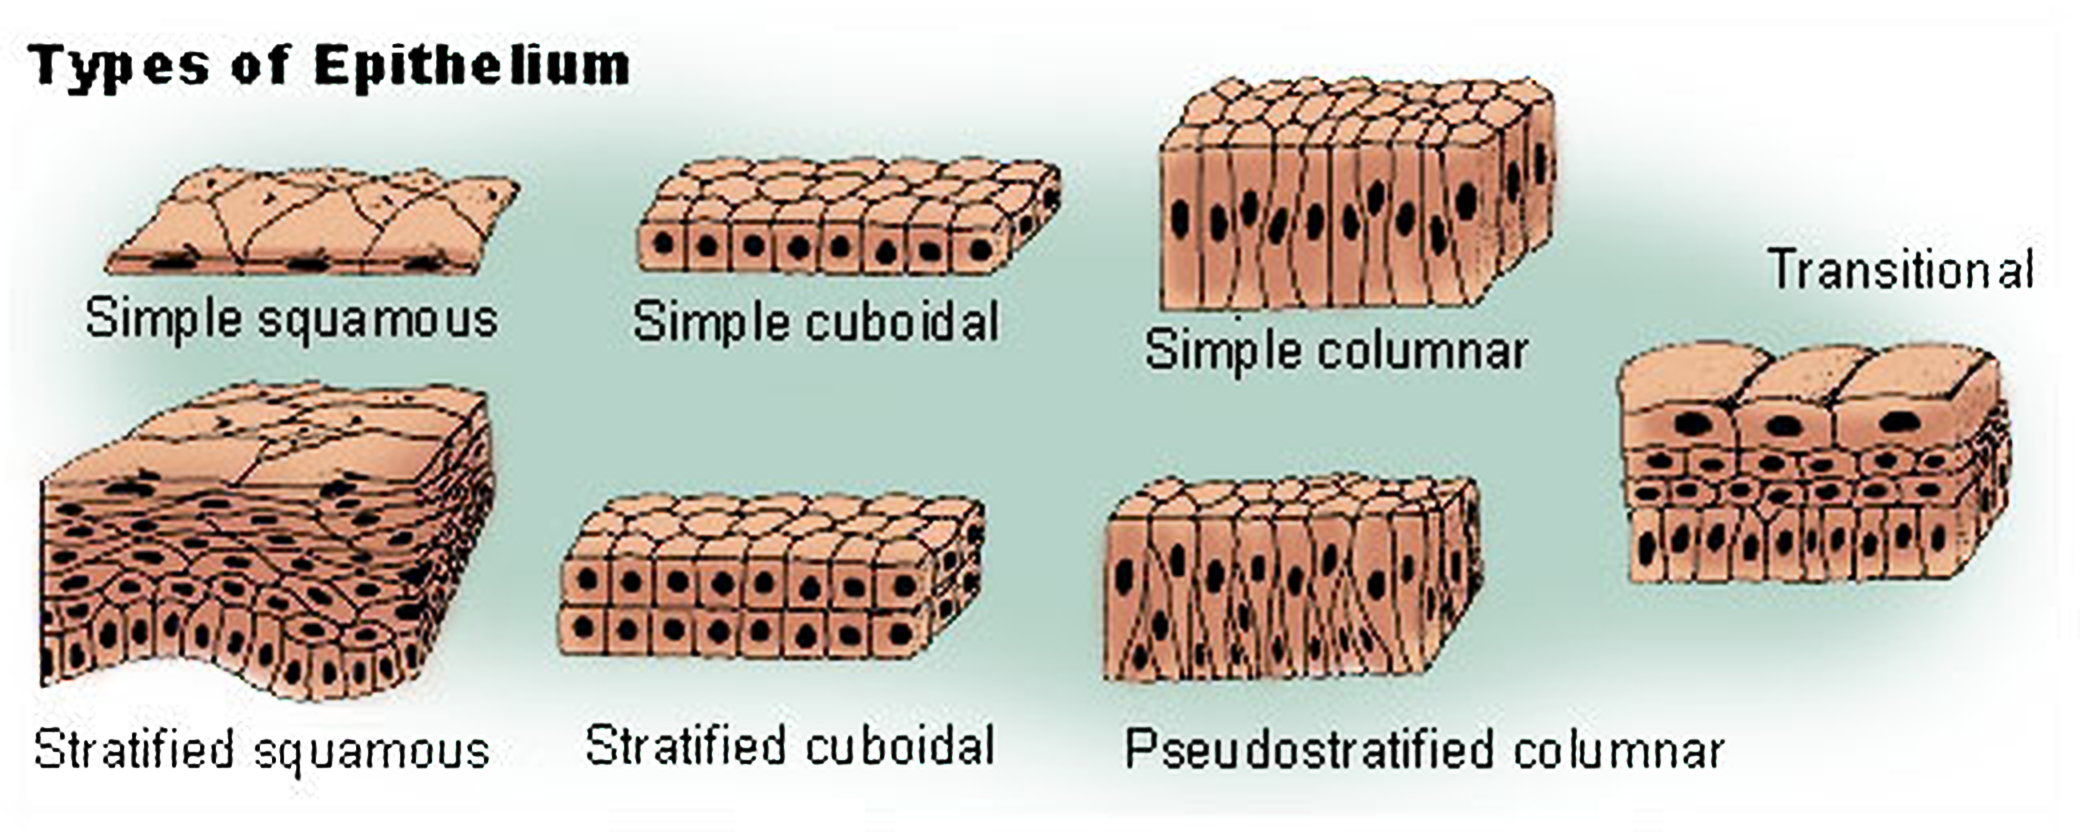
\includegraphics[width=\textwidth]{../diagrams/output.png}
\caption{The Types of Epithelial Tissue}
\label{fig:types}
\end{figure}

Botanical epithelia are rather simple and homogeneous - a single layer of cells covering exposed surfaces. As Figure~\ref{fig:types} shows, however, there are many types of epithelial tissue in animals which vary in the number of layers they include, how the cells are shaped, and how tall the cells are. Each of these types of cells are found in a different region of the body where they perform a specific function.  For example, the simple squamous epithelium is no more than one layer of cells thick, and the cells are all very flat, much flatter than they are wide. These cells are therefore well suited to  allow diffussion across themselves. As such, simple squamous tissue is found in the walls of blood vessels, and in the alveoli in the lungs, where the diffusion of oxygen occurs. On the other hand, columnar cells are much taller than they are wide, and are thus well suited to absorption. These cells are found in the intestines where they absorb nutrients from passing food. Stratified squamous epithelia are several layers thick line the esophogas and mouth and serve to protect against abraision.

What all of these tissues have in common, however, is how amenable they are to computational modeling. The simplest case is that of simple epithelia, which typically have near-uniform height, and very little difference in appearance between their apical and basal faces. This means that the cells can easily be approximated by two dimensional meshes, since the top and bottom of the cells move in tandem and the surface where two cells touch can be approximated by a line. Slightly more difficult is the modeling of stratified tissue. In this case, the tissue develops in three dimensions, since underlying cells affect the cells on top of them. These cannot be modeled in two dimensions, but can be modeled by a solid composed of three dimensional polytopes. The theory behind these models is well developed, but the techincal details of implementing such a model has made it so that very exist, and are often quite limited \footnote{Even a leading epithelial tissue simulator, Chaste, still does not have stable 3D modeling capabilities}. 

To give you an idea of what current epithelial tissue simulators have produced, I am putting some images from recent papers.

\begin{figure}[h]
    \centering
    \begin{subfigure}[b]{0.4\textwidth}
		\centering
		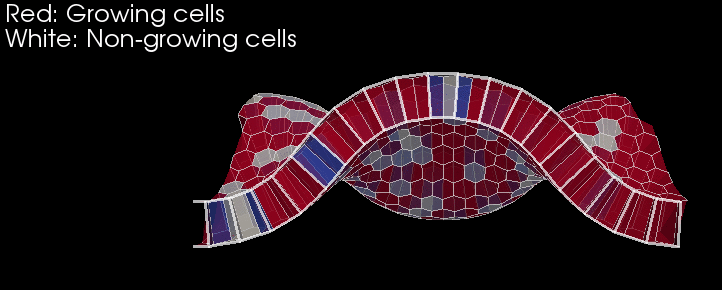
\includegraphics[width=\textwidth]{../diagrams/okuda1.png}
		\caption{Simple Squamous Tissue Bending in 3D\cite{Okuda1}}
		\label{fig:okuda1}
    \end{subfigure}
    \hfill
    \begin{subfigure}[b]{0.4\textwidth}
		\centering
		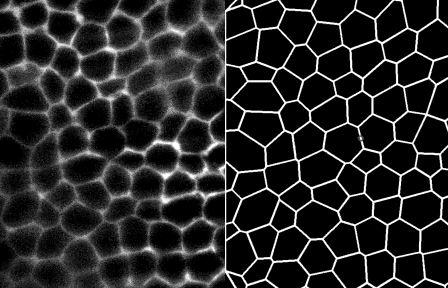
\includegraphics[width=\textwidth]{../diagrams/perfect.png}
		\caption{Comparison of Living Tissue and Simulation\cite{Yoshi}}
		\label{fig:yoshi}
    \end{subfigure}
    \hfill
    \begin{subfigure}[b]{0.4\textwidth}
        \centering
        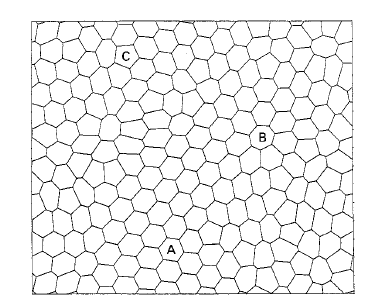
\includegraphics[width=\textwidth]{../diagrams/HondaResult.png}
        \caption{Equilibrium Mesh\cite{HondaNagai}}
        \label{fig:Honda}
    \end{subfigure}
    \hfill
    \begin{subfigure}[b]{0.4\textwidth}
        \centering
        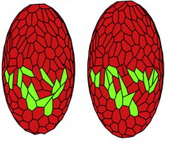
\includegraphics[width=\textwidth]{../diagrams/mirim.png}
        \caption{Equilibrium Mesh on a 3d Surface \cite{Vertex Models}}
        \label{fig:mirim}
    \end{subfigure}
    \caption{Some existing models of epithelial tissue.}
    \label{fig:four graphs}
\end{figure}


So, the question still remains: ``Why Study Epithelial Tissue?". The study of biological tissues has intrinsic value, much as mapping constellations or studying the properties of natural numbers. Beyond its inherent worth, current research in epithelial tissue is producing great results in the field of epithelial tissue  morphogenisis and diversifictation as well as wound healing. The Honda-Nagai model which we will discuss in great detail in this paper successfully reproduced the dynamics of the healing of wounds to cats' corneas\cite{Wound Healing}. This model has also been able to reproduce all of the essential dynamics of epithelial tissue \cite{HondaNagai}. So, in conclusion, we \emph{should} be modeling epithelial tissue computationally because it is easy to do, effective, an the community is currently very active and passionate about the field. 
\chapter{Overview of the Model}
\begin{center}
\emph{The world was so recent that many things still lacked names,}\\
\emph{and to mention them one had to point with a finger. }\\
\textbf{\hspace{10ex} - Gabriel Garcia Marquez}
\end{center}
\section{Introduction}
A two dimensional \textbf{vertex dynamics model} of epithelial tissue is made up of vertices and edges. A cell is represented as a convex hull made up of cells and vertices. This model presupposes that the movement of cells in epithelial tissue can be approximated by the movement of the vertices which make up the cell. Some force is hypothesized to be the guiding force between epithelial cell movement, and this force is applied to all of the vertices in the mesh of cells, producing some final state of the tissue. The three dimensional model is an extension of the two-dimensional model, but the mesh comes to include not only vertices and edges, but also cell faces. 

Epithelial vertex dynamics has been a lively field of research since the 1970s because of several heartening results in the field. Some researchers have had success modelling the morphogenesis of \emph{Drosophila} wing growth, whereas other researchers have successfully reproduced the dynamics of corneal wound healing. Unfortunately, these results have not come from one standard force, but from a variety of different hypothesized forces.

As an example of the different approaches to force modelling, let us consider the Weliky-Oster and Honda-Nagai forces. The Weliky-Oster model specifies explicit forces which act act upon the vertices due to a tension associated with boundary lengths. In two dimensions this constributes two tensions from each edge in a cell surrounding a vertex. The model also includes a cortical pressure due to the osmotic pressure inside a cell, which tends to push a vertex away from the interior. The Honda-Nagai Model (which I have recreated) takes a much different approach and instead specifies a potential energy function for the tissue. In this model the cells move passively as they attempt to minimize the potential energy of the tissue\cite{Vertex Models}. 

While both of these models successfully reproduce the topological and geometric properties of epithelial tissue, I have chosen to focus my efforts on the Nagai-Honda model. So, let us look at the model in some depth.

\section{The Nagai-Honda Model}
\subsection{How the Vertices Move}
A very basic result from physics is the relationship between force and potential energy, and this is one of the building blocks of the Nagai-Honda Model. Given a force vector $F$ and scalars $U$, for potential energy and $W$ for work, we can derive the relation:

\begin{gather}
\vec{F} = (F_x, F_y, F_z)\\
W = -\Delta U(\vec{x}) = \int_{x_0}^xF_xdx+\int_{y_0}^yF_ydy+\int_{z_0}^zF_zdz\\
\nabla(-\Delta U(\vec{x}) = \nabla\Bigg(\int_{x_0}^xF_xdx+\int_{y_0}^yF_ydy+\int_{z_0}^zF_zdz\Bigg)\\
-\nabla U(\vec{x}) = \vec{F}
\end{gather}

The second building block of the Nagai-Honda Model is the equation of motion. In 1989, K. Kawaski showed that the dynamics of grain growth can be reduced to a first order system given by:
\begin{equation}
\eta\frac{dr_i}{dt} = F_i
\end{equation}

where $F_i$ denotes the force applied to vertex $i$ and the left hand side is the velocity of the vertex multiplied by a positive drag coefficient, $\eta$\cite{1989 Kawasaki}.

\begin{figure}
\centering
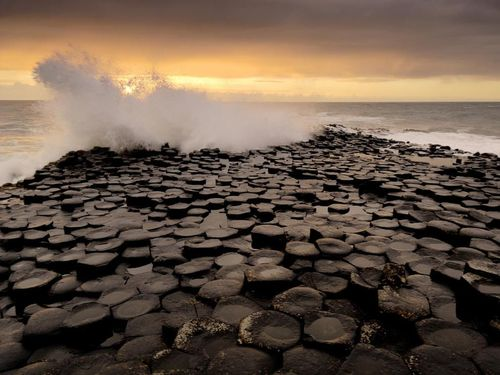
\includegraphics[width=0.5\textwidth]{../diagrams/resize_giant.jpg}
\caption{The Giant's Causeway}
\label{fig:cause}
\end{figure}

A very important paper in the field of natural cellular structures, of which the study of epithelial tissue is a small subset, is \emph{Soap, Cells, and Statistics}. In this paper, leading researchers in the field  argue that there must be some natural mechanism underlying the development of epithelial tissue, columnar basalt formations, soap froths, grin growths, and other cellular structures, as they exhibit a great deal of similarity. For example, consider the images of epithelial tissue presented throughout this paper next to the image of The Giant's Causeway in Northern Ireland. Some differences include the exact distribution of cell shapes, the presence of chemicals in biological tissues versus the absence of growth inducing chemicals in geological structures, and the active migration of biological cells versus the entirely passive movement of soap froths; still, the equilibrium patterns of these diverse structures leads one to believe that there must be some underlying principle. The Honda-Nagai model builds upon this idea and borrows ideas from the field of grain growth.

Putting these building blocks together, we have a force acting on the vertices in the mesh, and an equation of motion which explains how the vertices move. Now all that is needed is a free energy function from which to derive our force (and this force should be similar to the force found in other cellular structures). The free energy function which provides the applied force was taken in part from the grain growth model, which asserts that grains want to achieve a target volume and perimeter via some still unknown mechanism. As previously mentioned, biological cellls have idiosynchratic mechanisms working on them as well. As such, the model was extended to include a purely biological factor, \emph{differential adhesion}. It is well known that cells have a proclivity to attach more tightly to certain cells  than to others due to the presence of certain cadherin proteins in the membranes of the cells. This tendency is called differential adhesion.

The first two energy terms assume that the cell is elastic, and that the cell wants to return to a target shape. Therefore, the first two energy terms are of the elastic potential form: 
\begin{equation}
C(x-x_0)^2
\end{equation}
\begin{figure}
\centering
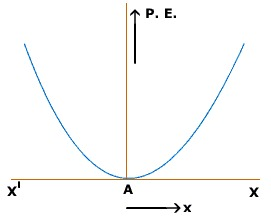
\includegraphics{../diagrams/pe.jpg}
\caption{Potential Energy as a Function of Distance from Equilibrium.}
\label{fig:pe}
\end{figure}
where $x$ is some physical quantity, and $C$ is some constant. The plot of this energy is therefore a parabola with a minimum at $x =  x_0$ ($A$ replaces $x_0$ in Figure~\ref{fig:pe}) and the farther $x$ is from $x_0$, the more potential energy there will be in the cell. 
The last energy term is an adhesion energy, which is proportional to the amount of interfacial surface area between a cell and its neighbor. Here are the three energy terms:
\begin{enumerate}
\item The deformation energy term \\ 
\begin{equation}
U_D = \lambda(A - A_0)^2
\end{equation}
 where $A_0$ is a target area for a cell, and lambda is some positive constant.
\item The membrane surface energy 
\begin{equation}
U_S = \beta(C - C_0)^2
\end{equation}
 where $C$ is the cell perimiter, and $C_0$ is a target perimeter.
\item The cell-cell adhesion energy 
\begin{equation}U_A = \displaystyle\sum\limits_{j = 1}^{n}\gamma_{j}d_{j}\end{equation}
where $n$ is the number of vertices in the cell, $\gamma$ is some constant for the boundary in question between one cell and another, and d is the distance between one vertex and the next in a counter clockwise fashion. Note that in two dimensins the boundary is a distance $d$, but in three dimensions it would have to be the area of a cell face. Also take note of the fact that the gamma term could be implemented in various ways. I have chosen to assign a ``stickiness'' to each cell, and then the gamma term is calculated as the average of the stickiness of the two cells.
\end{enumerate}

 As seen in \cite{ChasteMain}, this force on each vertex i is given by the negative gradient of the potential:

\begin{equation}
F_i = -\displaystyle\sum_{l\in N_i}(2\lambda(A_l - A_{0_l})\nabla_iA_l + 2\beta(C_l - C_{0_l})(\nabla_i d_{l, I_l-1}+\nabla_i d_{l, I_l}) + \gamma_{l, I_l-1}\nabla_i d_{l, I_l-1} + \gamma_{l, I_l}\nabla_i d_{l, I_l}
\end{equation} 
where l is the lth cell containing vertex $i$, given a counter clockwise orientation. $I_l$ is the local index of node $i$ in element $l$.

The way to derive this force is not described in much of the literature, and only is partially described in \cite{Chaste Main}. I will explain the force in some detail here.

 The area of a cell is given by Gauss's Shoelace Formula:
\begin{equation}
A = \frac12\Big|\sum\limits_{i=1}^N\Big(x_iy_{i+1}-x_{i+1}y_i\Big)\Big|
\end{equation}
where N+1 = 1. Therefore, the gradient is given by:
\begin{equation}
\nabla_i A_l = \frac12
\Big<
y^l_{I+1} - y^l_{I-1},\;\;x^l_{I-1} - x^l_{I+1}
\Big>
\end{equation}
 where the superscrpits $l$ denote that x, y are in cell $l$. The subscripts are local indices in the cell $l$, and the orientation of vertices is counterclockwise. The circumference is given by:

\begin{equation}
C = \sum\limits_{j=1}^Nd_j = \sum\limits_{j=1}^N\sqrt{(x_{j+1} - x_j)^2 + (y_{j+1} - y_j)^2}
\end{equation}
Therefore
\begin{gather}
\nabla_iC = \nabla_id_{i-1} + \nabla_id_i
\end{gather}

and

\begin{equation}
\nabla_id_{l, j} = \frac1{d_{l, j}}
\Big<
x_{j+1}- x_j,\;\; y_{j+1} - y_j
\Big>
\end{equation}

Substituting the above values into the equation:
\begin{equation}
-\nabla_iU = -\nabla_i(U_D + U_S + U_A) = F_i
\end{equation}

gives the force described above.

\subsection{Academic Dishonesty, or Obvious Modeling?}

I am not at the point yet in my understanding of the physics of epithelial tissue to comment upon whether this model ought to be intuitively obvious to the physicist, or whether it is a carefully chosen model which has discarded many extraneous possibilities. A recent article \cite{Julicher Cheats} gives the equation for the potential in the mesh as:
\begin{equation}
E_i = \sum\limits_{\alpha}\frac K2(A_\alpha - A_\alpha^0)^2 + \sum\limits_{i,j}\Lambda_{ij}l_{ij} + \sum\limits_{\alpha}\frac\Gamma2L_\alpha^2
\end{equation}
 Where $i$ denotes vertex i, $\alpha$ denotes a cell of which $i$ is on the border, the $A$ and $A_0$ terms denote area and target area, and the $l_{ij}$ denotes the length of the boundaries on which $i$ lies, and the $L$ denotes the perimeter. The H. Honda or T. Nagai are not cited in the bibliography to this paper by several well known and respected scientists, so either this model is so obviously adecuate that it isn't necessary to cite the original author, or this is a case of academic dishonesty.

\subsection{Topological Changes to the Mesh}
\begin{figure}{}
    \centering
    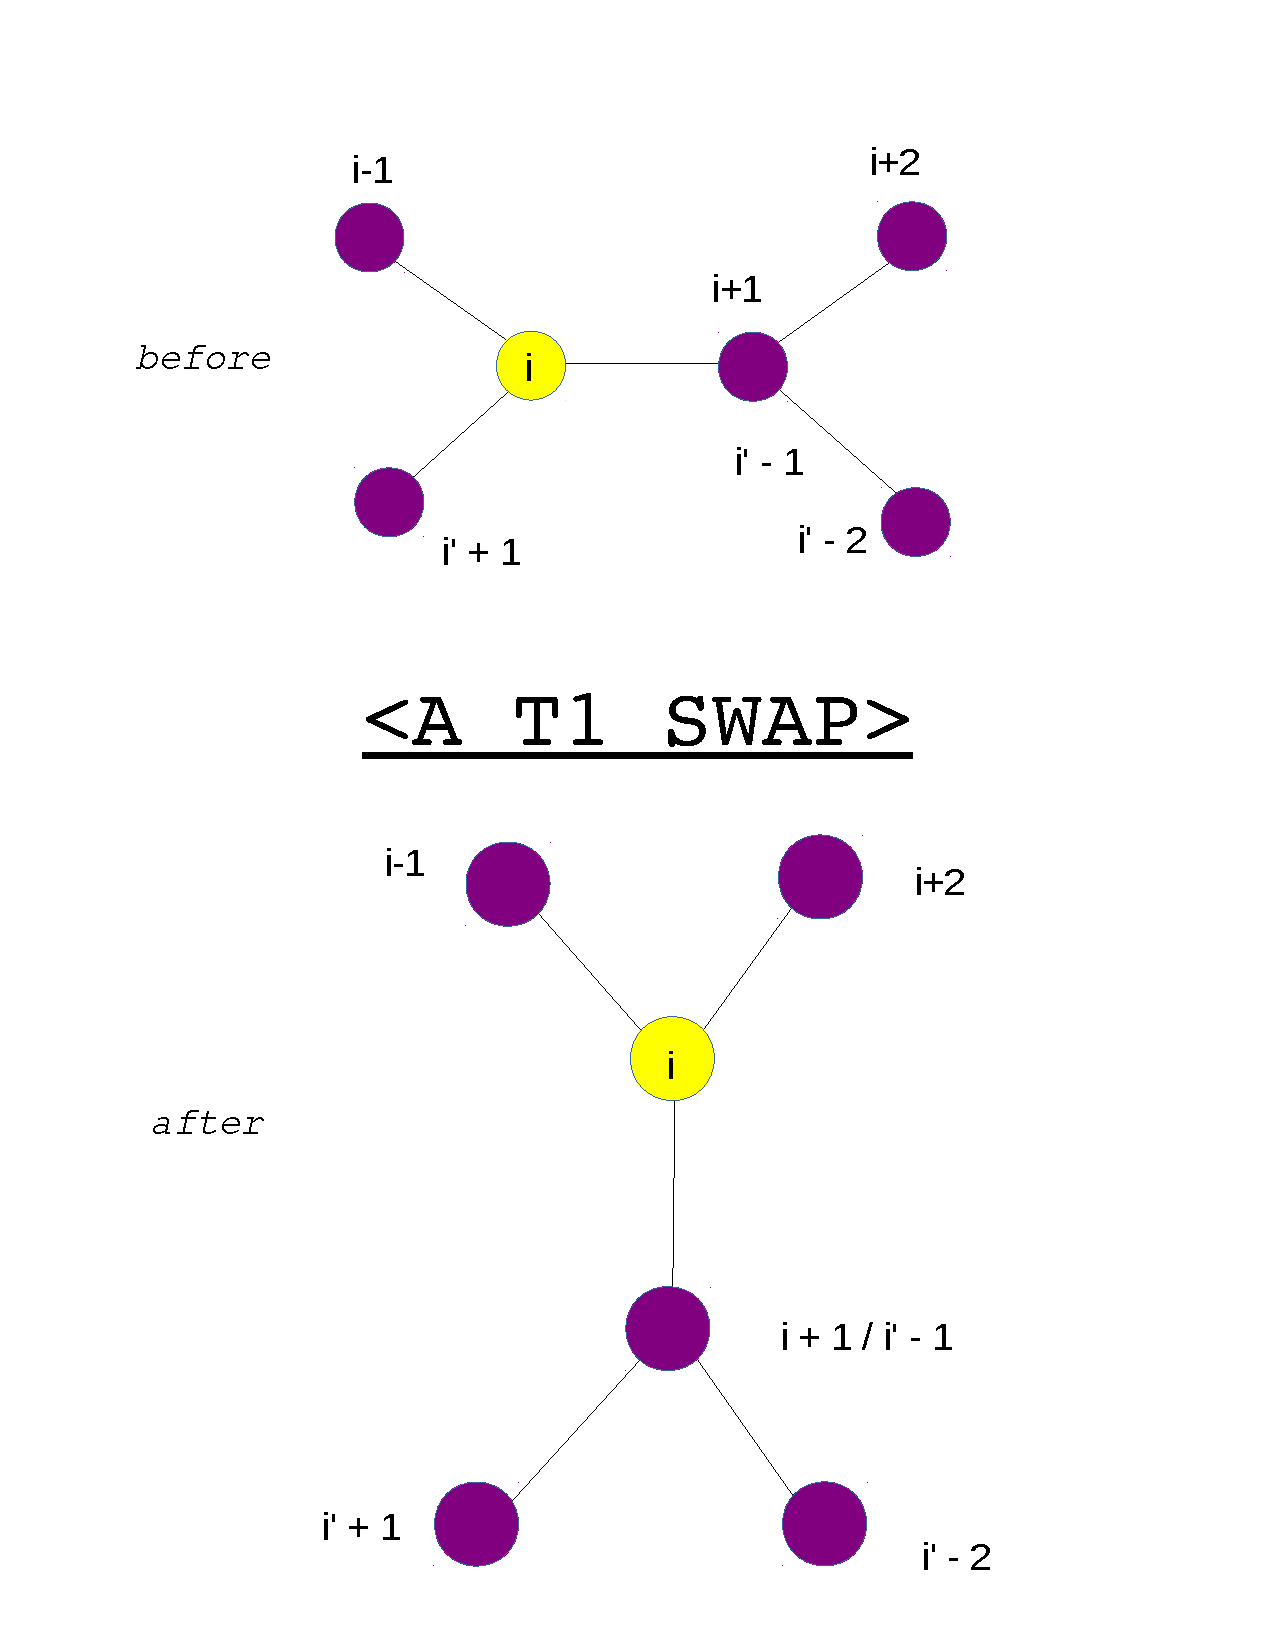
\includegraphics[width=\textwidth, height=0.8\textheight, keepaspectratio]{../diagrams/t1.pdf}
    \label{fig:t1}
    \caption[A T1 Swap]{A T1 Swap. The numbers reflect the counterclockwise storage of the vertices. The prime serves to distinguish an index in the top cell from an index in the bottom cell.}
\end{figure}
There is emprirical evidence that nearly all vertices in a sheet of epithelial tissue have degree three. Since the coordination number of the almost all vertices is three, this has led many modelers to consider what sort of topological changes can occur in mesh of these types of cells without changing the connectivity.  As it turns out, there are three changes which can occur.  The first is called a T1 swap and in illustrated in Figure~\ref{fig:t1}. This is also called a "neighbor exchanging swap" because, as you can see, two cells which were adjacent cease to be neighbors and two cells that weren't adjacent become neighbors. The T1 swap occurs when two vertices become critically close to each other, and instead of allowing the force to drive the vertices into each other we rotate their edge by 90 degree. In nature this sould correspond to two vertices getting very close, colliding, and then flattening out into an edge. Our model performs this action discretly as a simplifying measure, however, because otherwise for a moment a vertex would have degree four, and this would be difficult to handle with out a very complex data structure. The second topological change is the T2 swap, which is also known as the "cell removal swap." This occurs when a triangular cell becomes too small and is deleted and replaced by a single vertex. The last swap is cell division, occasionally referred to as the T3 swap. 

Cell division was not a part of the original Honda-Nagai Model, but it is now a very hot topic in computational tissue morphogenesis; it deserves mention. The challenge with implementing the T3 swap is that there are infinitely (within the bounds of floating point arithmetic) many choices about where to divide a cell, and there are several competing opinions (though no unanimouslly accepted theory) about how the dvision is oriented. Some cells divide along their longer axis, which is known as the `Hertwig's Long Axis Rule', but global tissue stress and local cell geometry are also thought to affect the orientation of cell division \cite{Order}\cite{Orientation}. The computational implementation of T3 swap is trivial, as the swap occurs by placing two new vertices in the interior of opposite edges and then connecting them by a new edge. The trouble is that it is not clear which edges ought to have vertices implanted, or where to insert these vertices, and the choice of where to divide a cell in a proliferating tissue can have profound effects upon the geometric appearance of a tissue \cite{Epithelial Topology}. There will be more discussion of cell division in the section of the paper dealing with the technical details of the implementation of \emph{Epithelium}.

\begin{figure}
\centering
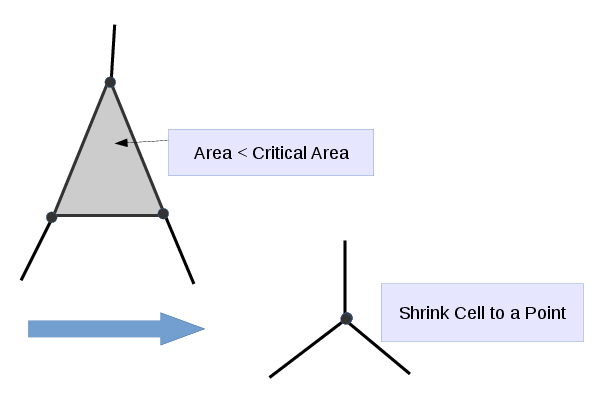
\includegraphics[width=0.5\textwidth]{../diagrams/T2swap.png}
\caption{A T2 Swap}
\label{fig:t2}
\end{figure}

\subsection{Quality, Not Quantity}

The equations in this model are dimensionless. I will not undertake a discussion of how to derive the dimensionless model from the dimensional model, but for the curious reader this is all laid out in \cite{HondaNagai}. Typically, one would not choose the values of the parameters $\alpha$, $\beta$ and $gamma$, but would instead have some dimensional biological data and go through the necessary conversion steps to convert these parameters to the simpler ones. Interestingly, in vertex dynamics literature I have read and cited in the bibliography, the only clearly stated parameters appear in \cite{ChasteMain}, and these are said to be taken from several papers which the authors (though I myself did not find these values explicity stated).  

There is little difference between equilibrium states in the Nagai-Honda model, as can be seen in the section of this paper dealing with the output of the code. Still, it has been shown that different parameter values coupled with other mesh changing operations (such as oriented cell division) can cause drastically different types of morphogenesis \cite{Overview}. For example, drosophila wings, with their highly oriented divisions, have been shown to contain approximately 80\% hexagonal cells whereas cucumber epidermis contains approximately 47\% hexagons \cite{Epithelial Topology}. While all epithelial tissue has a strong tendency towards achieving an equilibrium dominated by hexagons, the width of the distribution of cell shapes differs by cellular structure and, hence, by parameter choices \cite{Soap}. 

For those interested I have included in this paper charts which display the equilibrium meshes for different parameter values, along with a graph of the equilibrium distributions of cell sizes. These tables are found in chapter TITLE OF CHAPTER HERE. What you will see in the charts is that my implementation of the Honda-Nagai Model reproduces the results of the authors' original paper in that given a wide variety of parameterizations the mesh tends towards six sided cells. Here is one graphic from \cite{HondaNagai} in which they illustrate the distribution of cell shapes as a function of time. 

\begin{figure}
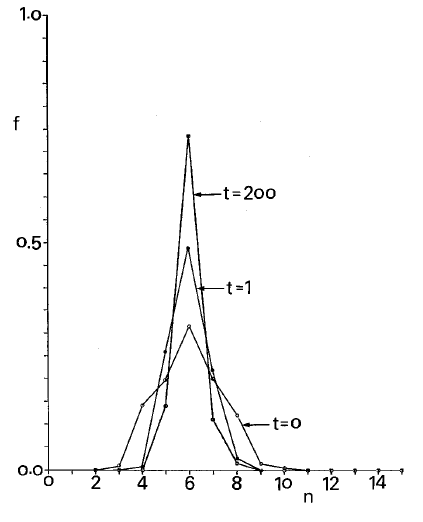
\includegraphics[width=0.5\textwidth]{../diagrams/distibutionHonda.png}
\caption{The Distribution of Cell Shapes As a Function of Time \cite{HondaNagai}}
\end{figure}

\chapter{Further Remarks About Epithelial Tissue and the Honda-Nagai Model}

\section{The Euler Characeteristic and Its Implications}
In this section I will expand upon some observations made in \cite{Soap}. \textbf{Euler's Formula} is an equation which relates the number of edges, faces, and vertices in a graph or polyhedron. An invariant $\chi$ relates the faces, edges, and vertices as follows:

\begin{equation}
\chi = V - F + E
\end{equation}

The invariant depends upon the graph or polyhedron in question. We will ignore the exact value of $\chi$ and comfort ourselves with the fact that it is a constant. The majority or current vertex dynamics models assume that vertices will have a coordination number of 3, and are based upon empirical results from biology. While there are certain models which consider \emph{rosettes}, for now we will assume that all vertices connect to exactly three other vertices. Then we notice that all edges have two vertices, and that all vertices are connected to three edges. Inititally, our intuition tells us that there should be three times as many edges as vertices, which leads us to the incorrect:
\begin{equation}
3V = E
\end{equation}
But then we notice that if we consider all of the vertices in the mesh, we count each edge twice, so we divide the conjectured  number of edges by two and then simplify to get:
\begin{equation}
3V = 2E
\end{equation}

Similarly, if we consider how to relate the number of edges to the faces in the mesh, we conjecture that the number of edges in equal to the number of cells with 3 sides plus the number of cells with 4 sides plus the number of cells with 5 sides plus . . . each multiplied by the number of edges per cell. THis gives us:
\begin{equation}
\sum_{k=3}^N kF_k = E
\end{equation}
Where $N$ is the highest number of edges encountered by any cell in the mesh. But in this way we have again counted all of the edges twice, so the true number of edges must be the summation above divided by 2. We simplify the equation to :
\begin{equation}
\sum_{k=3}^N kF_k = 2E
\end{equation}

Now, we are able to reduce Euler's Forula to one variable using the relationships given above.
\begin{gather}
V - F + E = \chi\\
\frac{2E}3 - F + E = \chi\\
\frac{5E}3 - F = \chi\\
\frac{\sum_{k=3}^N kF_k}{6} - F = \chi\\
(\frac{\sum_{k=3}^N kF_k}{F} - 6)F = 6\chi
\end{gather}
Biological cells are very small, and an epithelial tissue is composed of many [NUMBER?] cells, so we assume that $F\to\infty$ and then immediately notice that the expression in parentheses must tend to zero as F goes to infinity, or else the left hand side of the above equation will not approach the constant $6\chi$
So we know that the algebraic mean of the number of vertices per face must be 6. Of course we have no reason at this point to assume a distribution which guarantees that the majority of cells in the tissue will have exactly six edges and will not, say consist of a mixture of 5 and 7 sided cells. Nevertheless, empirical evidence shows a strong central tendency in the distribution of cell shapes. Whenever a cell tries to stray from the mean, there are means (such as a T3 swap, described in the next section) of recentering the distribution at 6 sides. 

\section{Why the Specified Topology Is Not Perfect}
The choice to impose degree three on each vertex is not one hundred percent consistent with nature, but has been a part of most models of epithelial tissue. This is because empirical evidence shows that the \emph{majority} of vertices in a tissue will have out degree three. It is a simplifying assumption that \emph{rosettes} (epithelial cells organized radially about one vertex which has degree greater than or equal to 4) do not change the global dynamics of the development of an epithelial tissue.  Recent computer vision developments \cite{rose} have made it easier to detect rosettes in epithelial tissue samples and may in the future provide information about the number of these formations, or evidence that rosettes are an important feature of epithelial tissue. 

\begin{figure}[hb]
\centering
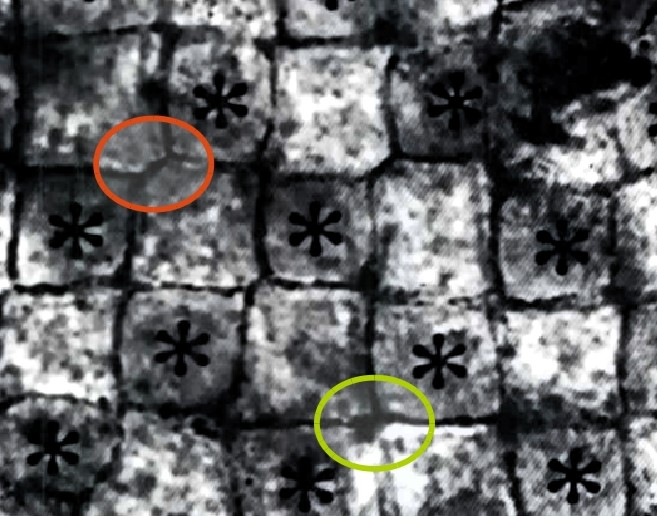
\includegraphics[width=0.5\textwidth]{../diagrams/checkers.jpg}
\caption[Square Cells.]{An image or Japanese quail epithelium. This tissue is patterned like a checkerboard and has been modeled in the past as a tissue with degree three vertices. It is possible that modelling this tissue as degree four vertices would provide better approximations of the dynamics.  In particular, notice that the orange vertices clearly can be modeled with degree three, wherease the green vertex could be one degree four vertex or two degree three.\cite{Checkers}}
\end{figure}


\section{Feedback Mechanisms and Proliferation}
This model is limited in that includes neither mechanical nor chemical feedback, and does not specify how cells proliferate. These are two extensions which can and have been made to the model by certain researchers. On the other hand, the dynamics of some successful models such as \cite{Morphogen} have the patterning of cells specified entirely by morphogens. In these models, chemicals called `morphogens' are what drive cells to proliferate, and the low concentrations of the morphogen on the fringe of the tissue explain why the tissue eventually ceases to grow as the tissue reaches a certain size.  Other models, such as those described in \cite{MechanicalFeedback} are based upon the vertex dynamics models such as the Honda-Nagai model, but include additional mechanical feedback terms which limit the growth of cells. 

\section{Additional Curiosities}
The vast majority of models assume that exactly three cells meet at any  vertex, except vertices on the boundary. In the language of topology, one would  say that all interior vertices in the tissue have degree three. Empirical observations show, however, that more more than three cells can meet at any junction under certain circumstances \cite{Vertex Models}. This means that models ought to be extended to include the formation of these `rosettes'.


\chapter{Epithelium}

\section{About Epithelium}
Here I present my implementation of the Honda-Nagai Model for epithelial tissue development as the simulation software called \emph{Epithelium}. The software is easy to install, takes up less than 50Mb, comes in parallel and non-parallel versions (Version 2.0.0, Version 1.0.0) and has very few dependencies. \emph{Epithelium} allows users to specify all parameters of interest in easily modifiable text configuration files, can handle simulations of arbitrarily large size, and can generate data for animations of epithelial tissue development as well as useful plots of important variables. 
\begin{figure}
\centering
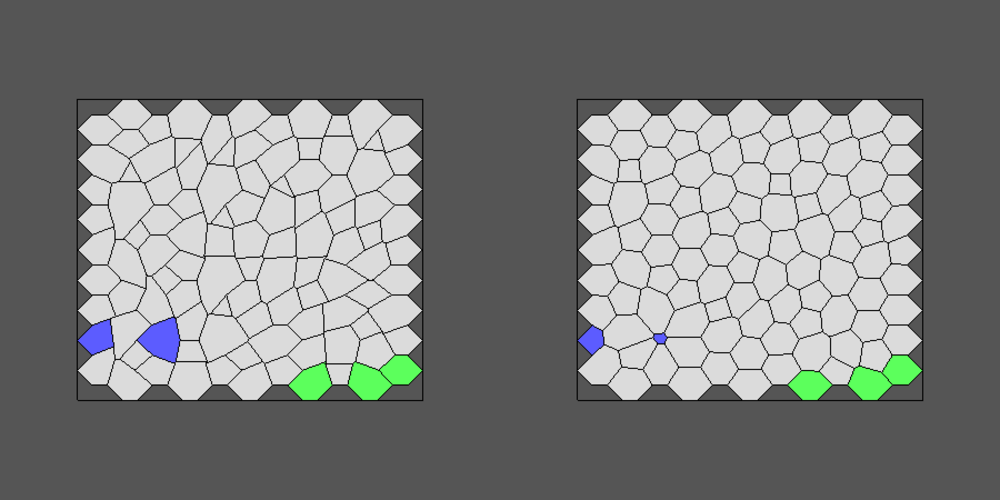
\includegraphics[width=\textwidth]{../diagrams/BeforeAfter.png}
\caption{Cells before (left) and after (right) the application of force.}
\label{fig:beforeafter}
\end{figure}
The source code is highly modularized and allows for ambitious users to easily extend the code to meet their needs. For example, alternate numerical integrators can easily replace the existing one, new mesh generators can replace the square mesh I have developed, and all data is output in space-separated formats which users with scripting language experience can transform to serve as input into the graphical utilities of their choice. In addition, the cell and coordinate classes are well documented and can be extended to output new data, as users may need. Figure~\ref{fig:beforeafter} provides a taste of the what the most basic installation of \emph{Epithlium} can do, showing a mesh of cells before and after equilibration.

\section{Sample Configuration Files}
The typical user will not want to modify source code, but would prefer to have a simple interface for changing simulation parameters. In this section we will explore in depth what the user interface looks like in terms of the three main configuration files, \texttt{config.txt}, \texttt{parameters.txt} and \texttt{change\_mesh.txt}.
\subsection{config.txt}
In this file, the user an specify some global properties about the mesh, and some important quantities for how the simulation will proceed. Most of the quantities are self explanatory. The \texttt{dimension} of the mesh refers to the number of cells along a given axis in a square mesh, and the \texttt{swap length} , \texttt{upper bound}, and \texttt{max swaps} parameters are used for performing random transformations to the mesh in the beginning of the simulation. The \textt{swap length} is the edge length below which a swap is performed. The \texttt{max swaps} parameter is the maximum nuber of random perturbations the code will make to the mesh before starting the simulation. The \texttt{upper bound} is an integer which is upper bound of the range for a random number generator. A random number generator produces a number in the range [1:\textt{upper bound}], and a random T1 swap is performed on `1'. The \texttt{delta} parameter specifies how close too vertices must be to force a T1 swap to occur.

OFF is the file format given to the plotting program \textbf{geomview} to plot the mesh. You can specify how often the code prints an image with the \texttt{frequency} parameter, but it must be a multiple of ten. More closely spaced images can be generated by using a smaller integration step size.
\begin{lstlisting}
13 # Dimension of mesh MUST BE ODD!!!!
0.01 # Maximum step size
1000 # Number of iterations
10 # frequency of OFF file output. Must be a multiple 10!
.1 # delta minimum vertex separation.
1000 # max swaps
1.5 # swap length
2 # upper bound random number generator
1 # Make energy and shape plots?
1 # Make a movie in the end? [1/0]
\end{lstlisting}

\subsection{parameters.txt}
In the \texttt{parameters.txt} file, the user can specify the parameters discussed in Chapter~\ref{chap:intro}. These are the default parameters for all of the cells in the tissue. 
\begin{lstlisting}
beta = 3;
lambda = 55;
t_gamma = 1;
t_area = 4.0;
\end{lstlisting}

\subsection{change\_mesh.txt}
While the parameters file allows global control of the mesh, the \texttt{change\_mesh.txt} file alows users to change local properties of the mesh. The first line of the file is for specifying how many $\gamma$, $A_0$, $\lambda$, and $\beta$ modifications will be made to the mesh. Note that $P_0$ cannot be changed, as $P_0$ is a function of $A_0$ (See Chapter~\ref{chap:intro}). The subsequent lines are for specifying the index and new value for each one of these modifications. As can be seen in Figure~\ref{fig:beforeafter}, cells can be color coded by parameter value to show these changes to the default settings.
\begin{lstlisting}
2 3 1 1 # num gamma, num area, num lambda, num beta
16 4.0  # gamma
17 5.1  # gamma
3 1.0   # area
4 1.0   # area
10 3.7  # area
1 10    # lambda
90 100  # beta
\end{lstlisting}

\section{Image Gallery}
Model parameters are easy to change in \emph{Epithelium}, and a variety of simulations are possible with very minimal effort on part of the user. Figure~\ref{figAFIHAoIHGa} - Figure~\ref{fig:aAIHgIASg} show the output from \emph{Epithelium} for several parameterizations. Each of the plots that follow show the decreasing energy in the mesh over time, the equilibrium distribution of cell areas, perimeters, and shapes. You may notice that there is very little variation between the plots - this is an essential property of the Honda-Nagai Model~\cite{HondaNagai} that the introduction of cell proliferation and an unbounded mesh could change.  

INSERT FIGURES

\section{The Design of \emph{Epithelium}}
The technical details of how a vertex dynamics model can be effectively implemented are not explained in great depth in the literature\footnote{\cite{ChasteMain} is an exception, but is rather advanced}. I will fill the void in this field in the section that follows and present a detailed look at the data structures and algorithms needed for the programming of the Honda-Nagai Model. It is fitting to start with a very high-level overview of the structure of the code.

\subsection{[Highly Simplified] Pseudocode}
Here I will briefly outline how the code works. All of the functions are explained in some detail later in this chapter.
\begin{lstlisting}
mesh_variables <- read_configs()
mesh <- make_mesh()
random_alterations(mesh)
copy(mesh, rotate_mesh)
rotate(rotate_mesh)
print(simulation_info) # So the user can verify all parameters.
for i = 1:num_iters
   if(iter%print_freq == 0)
      print(OFF_file)
   temp_mesh = NagaiHondaForce(mesh) 
   temp_rotate_mesh = NagaiHondaForce(rotate_mesh)
   mesh <- mesh + temp_mesh
   rotate_mesh <- rotate_mesh + temp_rotate_mesh
   performT2(mesh)
   performT1(mesh)
   performT2(temp_rotate_mesh)
   performT1(rotate_mesh)
rotate_back(rotate_mesh)
compare_mesh(mesh, rotate_mesh)
print(graphics and error analysis)
\end{lstlisting}

\subsection{Classes}
\emph{Epithelium} has a partially object oriented design. The cell and vertex classes organize the data into meaningul pieces.
\begin{itemize}
\item The {\color{red} Cell} class contains a number of useful functions and data members to make the code easy to read and understand. All cell information could have been stored in arrays, but the OO structure makes the code more readable. All cells know their index, which vertices (coordinates) make them up, they are able to calulate their area and perimeter, can modify their constituent vertices, can tell you whether or not ther contain a vertex, and can print out a graphical, color coded representation of themselves to an OFF file. Cells have other 
\begin{lstlisting}
public:
 cell(int index, vector$<$int$>$ AssociatedVertices,\
       double target_area = t_area, double gamma = t_gamma)
 {	
   assert(index $>$= 0);
   m_AssociatedVertices = AssociatedVertices;
   m_index = index;
   m_target_area = target_area;
   m_target_perimeter = sqrt(pi * m_target_area);
   m_gamma = gamma; 
 }
	
 cell(){} // Default constructor
	
 vector<int>GetVertices(){return m_AssociatedVertices;};
 int GetIndex(){return m_index;};
 void SetIndex(int index){m_index = index;};
 void SetTargetArea(double area){m_target_area = area;};
 double GetTargetArea(){return m_target_area;};
 double GetTargetPerimeter(){return m_target_perimeter;};
 double ComputeArea(double * X, double * Y);
 double ComputePerimeter(double * X, double * Y);
 void PrintCell(ofstream &OffFile);
 int ContainsVertex(int index);
 void SetGamma(double gamma){m_gamma = gamma;};
 double GetGamma(){return m_gamma;};
 void InsertVert(int v1, int v2);
 void EraseVert(int index)
 {
   vector<int>::iterator it = find(m_AssociatedVertices, index); 
   m_AssociatedVertices.erase(it);
 };
 void ReplaceVert(int before, int after)
 {
   vector<int>::iterator it = find(m_AssociatedVertices, before); 
   *it = after;
 };
 void SetVertices(vector<int> vertices)
 {
   m_AssociatedVertices = vertices;
 };
 int GetNumSides(){return m_AssociatedVertices.size();};
private:
 vector<int> m_AssociatedVertices; // Stored counterclockwise
 int m_index;	
 double m_target_area;
 double m_target_perimeter;
 double m_gamma;
};

\end{lstlisting}

\item{The Vertex Class}
The {\color{green} Vertex} class stores the index of a vertex, and 
whether or not the vertex will move during the integration. While a 
vertex object does not store the location of the vertex, it tells the 
simulator whether or not a vertex is on the border of a mesh and, if it 
is not, it is allowed to move. It was a design choice that 
\emph{Epithelium} be able to run three popular types of meshes, those 
with border, those without, and those that cover a surface.  Another 
benefit of the vertex class is that is allows users to easily extend 
the code to include forces acting on individual vertices, and to 
specify other types of vertices besides interior and exterior. The 
vertex class could be extended to include a member function such as 
activeMigration(), or any number of interesting functions. This code was developed with eyes to the future. 
\begin{lstlisting}
class vertex
{
public:
  vertex(int idx, bool t) : index(idx), IsInner(t){};
  vertex(){index = -1; IsInner = 0;};
  int index;
  bool IsInner;
  inline bool operator==(const vertex& rhs)
  {return index == rhs.index;};
};
\end{lstlisting}
\end{itemize}


\section{A Relational Database}
There is one other major idea behind the design of \emph{Epithelium}. A 
popular way to store data since the 1970's is to store data in groups of tables which are connected via \emph{keys}. This type of database is popular for reasons which will become apparent by means of a simple example. 

Consider a business which sells a number of products, and wants to keep 
track of their customers, the customer's orders, the customer's 
addresses, and information about the products ordered. A wasteful way 
to store this data is to create a large table in which the first column 
is for customer names. Next to every customer's name is the customer's 
address, and next to the customers address is the customer's order 
number. Next to the customer's order number is an item in that order, 
and next to each item ordered is the item information. This method of 
storing data is terribly redundant, because for each order with more 
than one item you would have redundant storage of the orderid, and of 
the customer information. Furthermore, every time the same item is 
order 

A better idea is to break this data up into several tables which 
together define a \emph{schema}. In the preceding example, the following tables define a good schema:
\begin{figure}
\centering
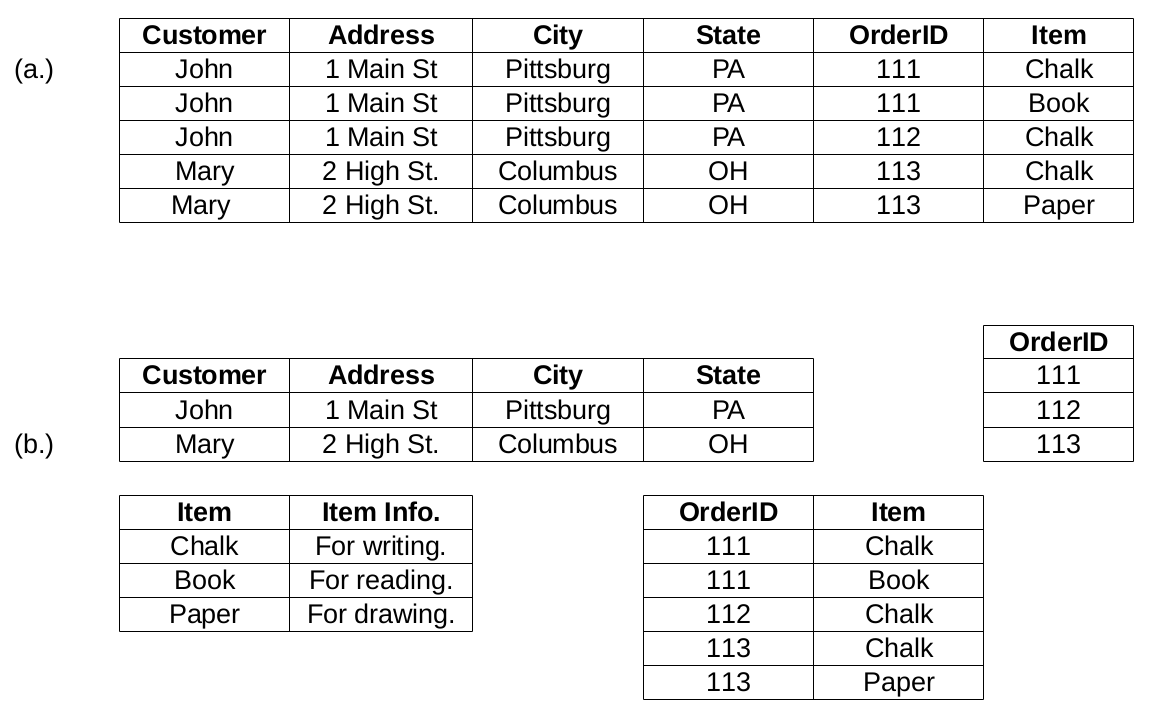
\includegraphics[width=\textwidth]{../diagrams/relationaldb.png}
\caption{An example of a relational database.}
\label{fig:rdb}
\end{figure}


We are now guaranteed that the customer information is not duplicated for every item in an order, and that item information is not duplicated every time an item is in an order.

\begin{figure}[h]
\centering
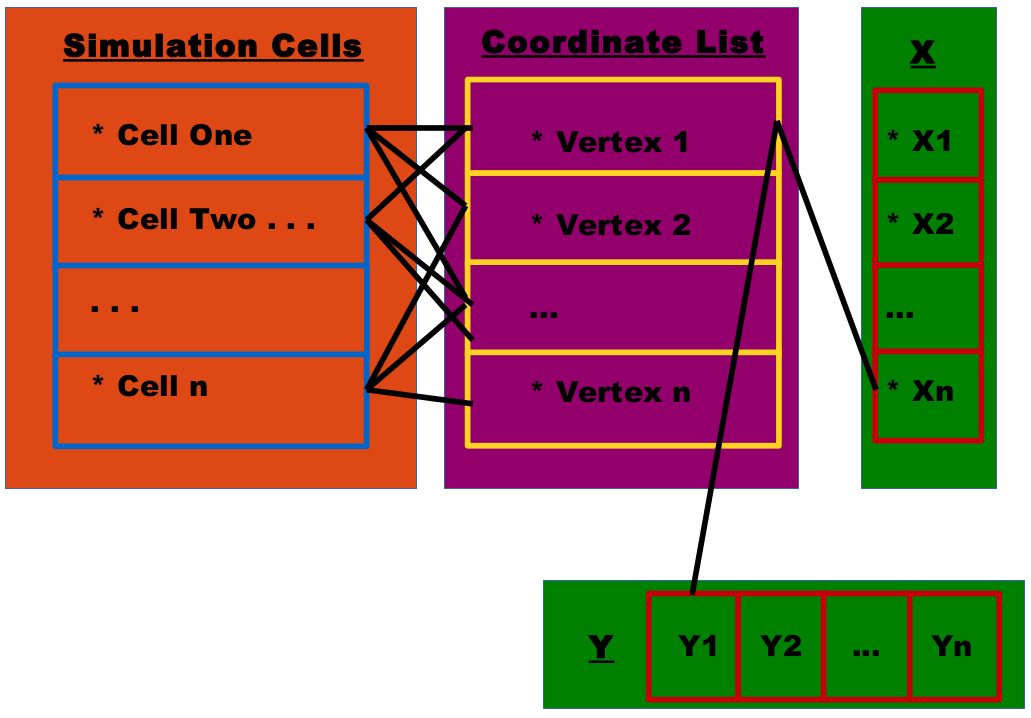
\includegraphics[width=0.5\textwidth]{../diagrams/ds.png}
\caption{\textbf{The Relational Database.}}
\end{figure}

My data structure is inspired by the relational database model. I have six tables, including the simulationCells, coordinateList, X, Y, tempX and tempY tables. The cell and coordinate tables are implemented as 1d vectors of cell and coordinate indices, whereas the position tables are implemented as 1d arrays for ease of passing these structures to CUDA C functions (will talk more about CUDA C later). The cells can extract coordinate information from the coordinateList table via the \emph{index} key, and the coordinateList can access the position information from the X and Y arrays via their own \emph{index}. The temporary X and Y arrays store temporary position information about the vertices before the mesh positions are updated. This choice saves memory because the cells, coordinates, and coordinate locations are stored independently of each other, and there is no data redundancy. 

\section{Initial Mesh Design}
The hex\_mesh() function generates an $n$x$n$ mesh of cells, where the 
dimension represents the number of cells touching the boundary in 
either axial direction. Figure ~\ref{fig:mesh} shows the default mesh 
used by \emph{Epithelium}, with the cell ids and vertex indices are 
labelled. After a sheet of cells is generated by 
hex\_mesh(), the tissue is perturbed in by first performing random 
T1 swaps on edges of the mesh, and then by perturbing the locations of a select 
number of vertices.

\begin{figure}
\centering
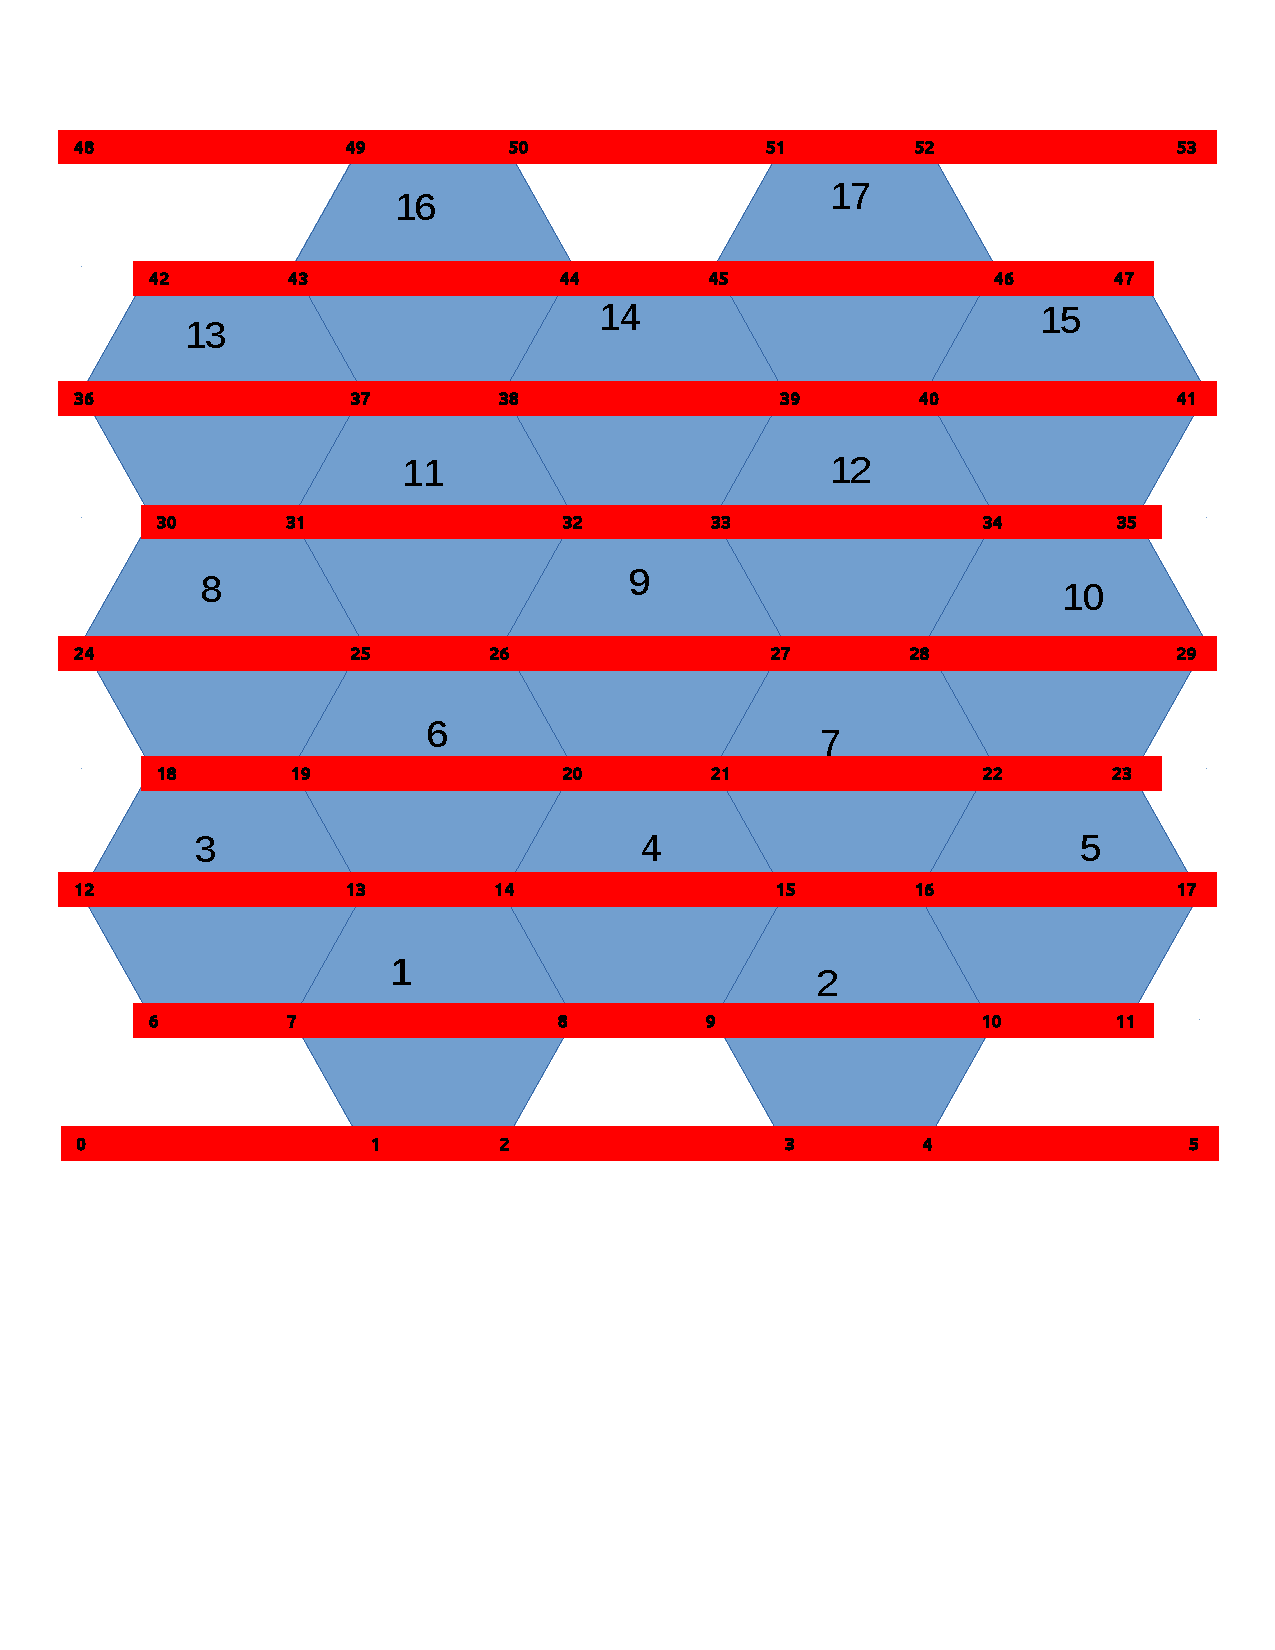
\includegraphics[height=0.7\textheight]{../diagrams/vert_mesh.pdf}
\caption[A 5x5 Hexagonal Mesh.]{\textbf{A 5x5 hexagonal mesh. The cell 
indices are written in the cells and the vertex indices are written on the red bars.}}
\label{fig:mesh}
\end{figure}
\section{Moving the Vertices}
\emph{Epithelium} loops over the vertices, computes the force applied to each vertex and then computes a displacement due to the force using the Euler Method. In their original paper, H. Honda and T. Nagai described the use of a Modified Runge Kutta Method to move the vertices, but this method would result in extra unnecessary computations at each time step. The \emph{Error Tolerance} section of this chapter describes how the Euler Method is numerically stable enough for this application. The same decision to use then Euler Method was made by the research group at Oxford that developed CHASTE, the \emph{other} leading software for implementing the Nagai-Honda Model. 

A displacement is calculated and stored in the temporary X and Y arrays. No vertex is permitted to move more than one half of the minimum delta separating vertices (the $\delta$ under which a T1 swap will occur) during an integration. By imposing this restiction we are ensuring that we will not miss the event of two vertices coming critcally close and a T1 swap occurring. Also, this prevents vertices from passing each other and invalidating the mesh. To ensure that no vertex moves too much, we store verify each displacement as we put it in the temporary X and Y arrays. If a displacement is too large, then the entire array of temporary displacements is erased, the time step is halved, and we begin the integration again. We could label the integrator as `fault tolerant'.

\begin{wrapfigure}{L}{0.4\textwidth}
\begin{center}
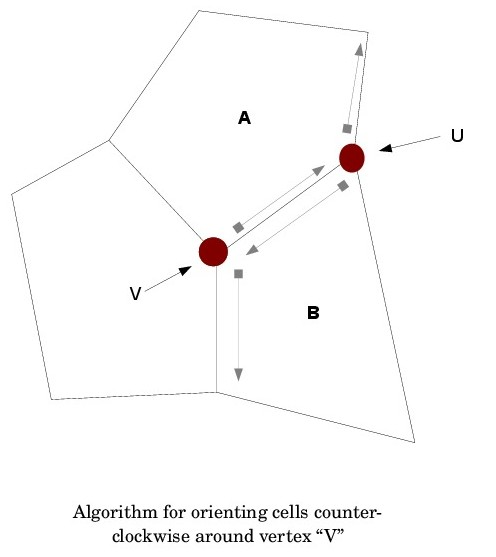
\includegraphics[width=0.38\textwidth]{../diagrams/counterclockwise.jpg}
\end{center}
\caption{Getting Cells in Order}
\label{fig:ctrclockwise}
\end{wrapfigure}

Another important aspect of the numerical integration is that cell and vertex information must be processed in counterclockwise order. In Figure~\ref{fig:ctrclockwise} I illustrate how a vertex can find the cells surrounding it in this order. When we are integrating a vertex $i$, the vertex first searches in the cell vector for a cell which contains it, and then the vertex finds the next vertex in that cell. Then, we have an edge. Some other cell contains that edge if it contains both of the vertices. That cell must be clockwise from the first. The cells are stored in the reverse order of which they are uncovered by this algorithm before the integration starts. This is a very expensive step ($O(n^3)$) in the computation, and ought to be optimized.


\section{Embarassing Parallelism and CUDA}
The numerical integrations and the vertex location updates exhibit what Cleve Moler describes as ``embarassing parallelism''. Computing the displacement of vertex \emph{a} does not depend upon the computation of the displacement of vertex \emph{b} during a given time step. Similarly, the vertex locations can all be updated in parallel since the update is simply a vector sum operation of the X and Y arrays with the temporary X and Y arrays, respectively. 

A popular hardware choice for parallel programming in last decade has been the NVIDIA GPU. CUDA is the NVIDIA extension of the C programming language which can run certain parts of C code on the GPU, while still running the serial and i/o operation on the CPU. I wrote some parts of the code in this language, and these parts were very simple to implement. The GPU is a collection of small processors, and the vertices are small, simple objects, so I mapped each vertex in the mesh to one of the hundreds of small processors to get some computational speedup.

Specifically, CUDA was employed to update vertex locations, since the sum of 1d arrays is well suited to a GPU. I also parallelized the rotation of the mesh and the reduction step which found the maximum error between the mesh and the rotated mesh. An interesting possibility is that of parallelizing the force computations. I was unable to do this with the code as it is because the cell data uses C++ vectors, while cuda only likes to take large C arrays as input. There is an interesting library called \emph{thrust} which can strips the vectors down to arrays and does all of the memory allocations for you, but the issue then becomes one of compiling the cells into one big vector with clever structure. This is left as a future project. 

CUDA was used to multiply each vertex in the mesh by the rotation matrix:
\[ \left( \begin{array}{cc}
\cos\theta & -\sin\theta \\
\sin\theta & \cos\theta 
\end{array} \right)\] 

\section{Computing Topological changes.}
\subsection{The T1 Swap}
The PerformT1s() function loops over all of the cells in the mesh, and checks the edge lengths in that cell. If an edge is critically small, then the other three cells involved in the junction are found. One of the two clashing vertices is deleted from the main cell, and the other clashing vertex is deleted from the neighboring cell. The midpoint of the critical edge is calculated, and then a perpendicular line is drawn through it. The vertices are then moved a distance $\delta/2$ into the interior of the cells ($\delta$ is the minimum vertex separation, and the vertices now have this minimal spacing). Then, these two vertices are inserted into the cells which previously hadn't been neighbors, making then adjacent after the swap. Figure ~\ref{fig:t1} offers a visual aid to understanding the swap. 

There are 8 cases to consider when inserting moving the vertices the distance $\delta/2$. I and Ip1 are the critically close vertices, where Ip1 comes before I in clockwise order in a cell. $mp$ is the midpoint of $\bar{(I, Ip1)}$. $dx$ and $dy$ are the displacements which will give a minimal separation after the swap. 
\begin{enumerate}
\item %1
\textbf{Given:}\\
I.x $<$ Ip1.x AND I.y == Ip1.y
\textbf{Then:}\\
I $\mapsto$ mp + (0, -dy) AND Ip1 $\mapsto$ mp + (0, dy)
\item %2
\textbf{Given:}\\
I.x $>$ Ip1.x AND I.y == Ip1.y
\textbf{Then:}\\
I $\mapsto$ mp + (0, dy) AND Ip1 $\mapsto$ mp + (0, -dy)
%%%%%%%%%%%%%%%%%%%%%%%%%%%%%%%%%%%%%%%%%%%%%%%%%%%%%%%%%%%
\item %3
\textbf{Given:}\\
I.x $<$ Ip1.x AND I.y $<$ Ip1.y
\textbf{Then:}\\
I $\mapsto$ mp + (dx, -dy) AND Ip1 $\mapsto$ mp + (-dx, dy)
\item %4
\textbf{Given:}\\
I.x $>$ Ip1.x AND I.y $>$ Ip1.y
\textbf{Then:}\\
I $\mapsto$ mp + (-dx, dy) AND Ip1 $\mapsto$ mp + (dx, -dy)
%%%%%%%%%%%%%%%%%%%%%%%%%%%%%%%%%%%%%%%%%%%%%%%%%%%%%%%%%%%
\item %5
\textbf{Given:}\\
I.x $<$ Ip1.x AND I.y $>$ Ip1.y
\textbf{Then:}\\
I $\mapsto$ mp + (-dx, -dy) AND Ip1 $\mapsto$ mp + (dx, dy)
\item %6
\textbf{Given:}\\
I.x $>$ Ip1.x AND I.y $<$ Ip1.y
\textbf{Then:}\\
I $\mapsto$ mp + (dx, dy) AND Ip1 $\mapsto$ mp + (-dx, -dy)
%%%%%%%%%%%%%%%%%%%%%%%%%%%%%%%%%%%%%%%%%%%%%%%%%%%%%%%%%%%
\item %7
\textbf{Given:}\\
I.x == Ip1.x AND I.y $>$ Ip1.y
\textbf{Then:}\\
I $\mapsto$ mp + (dx, -dy) AND Ip1 $\mapsto$ mp + (-dx, dy)
\item %8
\textbf{Given:}\\
I.x == Ip1.x AND I.y $<$ Ip1.y
\textbf{Then:}\\
I $\mapsto$ mp + (dx, -dy) AND Ip1 $\mapsto$ mp + (-dx, dy)
\end{enumerate}

\subsection{The implementation of the T2 swap.}
The PerformT2s() function looks at every cell in the mesh and checks its area. If the area is critically small, then the cell is deleted from the mesh. The centroid of the triangle is calculated, and this become the collapsed triangle. Then, one of the three vertices has its position updated to the centroid coordinate and any cell which contained on of the other two coordinates is assigned the centroid coordinate index as a replacement.

\section{Error Tolerance of the Algorithm}
\emph{Epithelium} has been empirically shown to be numerically stable; the code outputs an error measurement at the end of a simulation to give the user a sense of the stability. There was no clear way to provide an analytical proof of stability but at least we will always have an error measure to strengthen our confidence in the code. \emph{Epithelium} runs two simultions at the same time, one on the mesh made by hex\_mesh(), and another on the same mesh which has been rotated 45 degrees. Then, at the end of a simulation, the rotated mesh is rotated back and corresponding vertices are compared by index using the Euclidean norm. In practice we see near machine epsilon error for every simulation.

\begin{figure}[hr]
\centering
\includegraphics[width=0.5\textwidth]{../diagrams/rotate.png}
\caption{A Rotated Mesh for Error Analysis.}
\end{figure}

\chapter{The Design of \emph{GrowFlesh}}
In this chapter I will explain the internals of \emph{GrowFlesh}. I will outline the data structure I used for the model, and some of the interesting algorithms I desinged to calculate inter- and intra- cellular forces. It is interesting to note that a number of datastructures and algorithms were scrapped in the beginning of the modeling process because of the complicated relationship between and vertices. The model I have implemented is a vertex dynamics model, and, as such, one would think that the main object of interest should be a vertex. Vertices require information about the cells which contain them in order to be moved. With this as a starting idea, I developed a sophisticated vertex class which contained cells as member variables. Apart from the software bloat coming from many vertices containing massive amounts of cell information, another issue was that cells are made of vertices, and, as such, cells ought to contain vertices as member variables! Unfortunately this bilateral inclusion is not supported by C++. In this chapter I will describe how this issue was circumvented through the use of tables which mimic the behavior of a relational database.

\section{[Highly Simplified] Pseudocode}
Here I will briefly outline how the code works. All of the functions are explained in some detail later in this chapter.
\begin{lstlisting}
mesh_variables $<$- read_configs()
mesh $<$- make_mesh()
random_alterations(mesh)
copy(mesh, rotate_mesh)
rotate(rotate_mesh)
print(simulation_info) # So the user can verify all parameters.
for i = 1:num_iters
   if(iter%print_freq == 0)
      print(OFF_file)
   temp_mesh = NagaiHondaForce(mesh) # if any displacement in temp_mesh,
                                     # the displacement is recalculated
   temp_rotate_mesh = NagaiHondaForce(rotate_mesh)
   mesh $<$- mesh + temp_mesh
   rotate_mesh $<$- rotate_mesh + temp_rotate_mesh
   performT1(mesh)
   performT2(mesh)
   performT1(rotate_mesh)
   performT2(temp_rotate_mesh)
rotate_back(rotate_mesh)
compare_mesh(mesh, rotate_mesh)
print(graphs and error analysis)
\end{lstlisting}

\section{Classes}
\emph{GrowFlesh} uses two classes to organize data. They are the cell and coordinate classes.
\subsection{The Cell Class}
The cell class contains a number of useful functions and data members to make the code easy to read and understand. All cell information could have been stored in arrays, but the OO structure makes the code more readable. All cells know their index, which vertices (coordinates) make them up, they are able to calulate their area and perimeter, can modify their constituent vertices, can tell you whether or not ther contain a vertex, and can print out a graphical, color coded representation of themselves to an OFF file.
\begin{lstlisting}
public:
 cell(int index, vector$<$int$>$ AssociatedVertices,\
       double target_area = t_area, double gamma = t_gamma)
 {	
   assert(index $>$= 0);
   m_AssociatedVertices = AssociatedVertices;
   m_index = index;
   m_target_area = target_area;
   m_target_perimeter = sqrt(pi * m_target_area);
   m_gamma = gamma; 
 }
	
 cell(){} // Default constructor
	
 vector$<$int$>$ GetVertices(){return m_AssociatedVertices;};
 int GetIndex(){return m_index;};
 void SetIndex(int index){m_index = index;};
 void SetTargetArea(double area){m_target_area = area;};
 double GetTargetArea(){return m_target_area;};
 double GetTargetPerimeter(){return m_target_perimeter;};
 double ComputeArea(double * X, double * Y);
 double ComputePerimeter(double * X, double * Y);
 void PrintCell(ofstream &OffFile);
 int ContainsVertex(int index);
 void SetGamma(double gamma){m_gamma = gamma;};
 double GetGamma(){return m_gamma;};
 void InsertVert(int v1, int v2);
 void EraseVert(int index)
 {
   vector$<$int$>$::iterator it = find(m_AssociatedVertices, index); 
   m_AssociatedVertices.erase(it);
 };
 void ReplaceVert(int before, int after)
 {
   vector$<$int$>$::iterator it = find(m_AssociatedVertices, before); 
   *it = after;
 };
 void SetVertices(vector$<$int$>$ vertices)
 {
   m_AssociatedVertices = vertices;
 };
 int GetNumSides(){return m_AssociatedVertices.size();};
private:
 vector$<$int$>$ m_AssociatedVertices; // Stored counterclockwise
 int m_index;	
 double m_target_area;
 double m_target_perimeter;
 double m_gamma;
};

\end{lstlisting}

\subsection{The Coordinate Class}
The coordinate class stores the index of a coordinate, and whether or not the vertex will move during the integration. \emph{GrowFlesh} will run with two types of meshes: meshes with border, and meshes without. A mesh with border is a mesh with fixed border elements. A mesh without border is a mesh which was generated with periodic boundary conditions and which maintains the periodicity throughout the calculations done by the program. Border vertices will not move, whereas interior vertices will be able to move; the coordinate class allows us to secify whether or not a vertex is interior or exterior. Another benefit of this class is that is allows use to easily extend the code to include forces acting on individual vertices, and to specify other types of vertices besides interior and exterior. This code was developed with eyes to the future. Another interesting idea to explore in computational biology is active cell migration, ad the cell class allows us to specify which vertices want to move actively.
\begin{lstlisting}
class coordinate
{
public:
  coordinate(int idx, bool t) : index(idx), IsInner(t){};
  coordinate(){index = -1; IsInner = 0;};
  int index;
  bool IsInner;
  inline bool operator==(const coordinate& rhs)
  {return index == rhs.index;};
};
\end{lstlisting}

\section{Initial Mesh Design}
The hex\_mesh() function generates an $n$x$n$ mesh of cells, where the dimension represents the number of cells touching the boundary. 

\begin{figure}
\centering
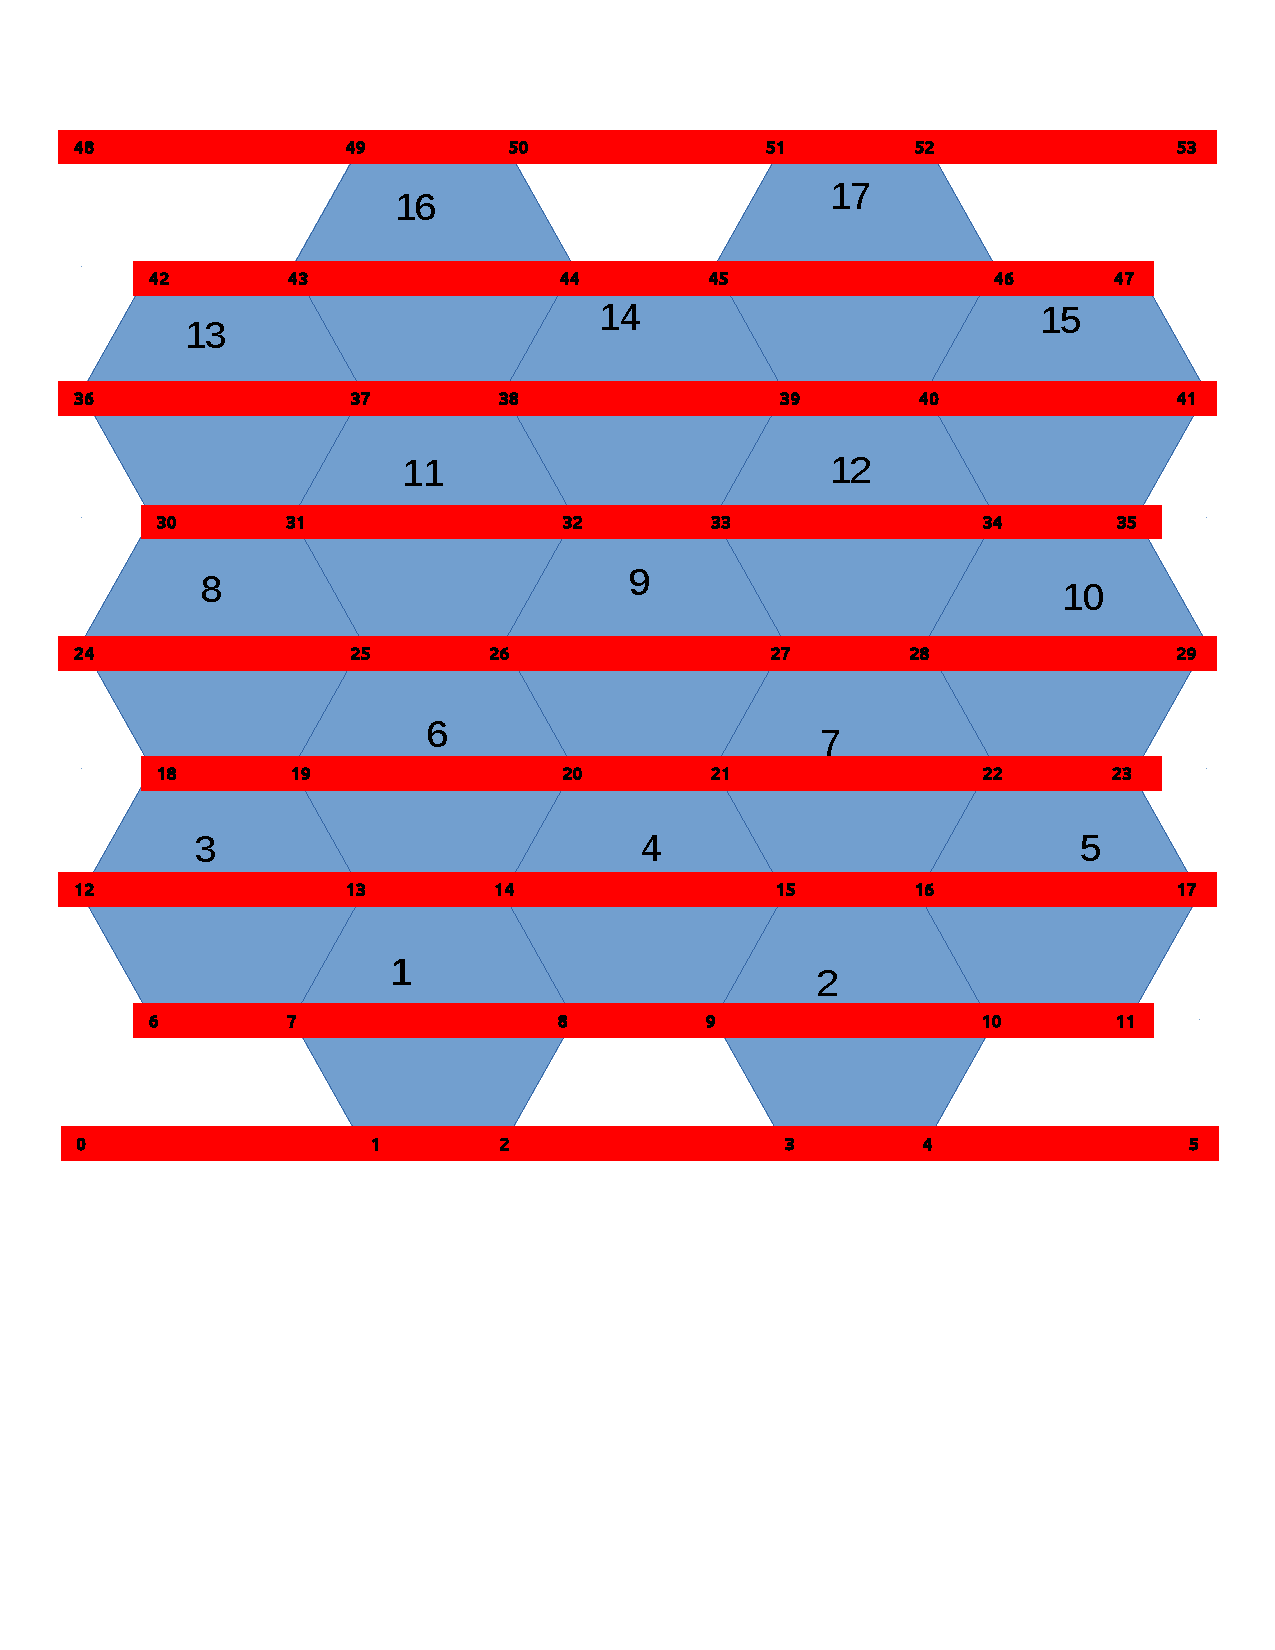
\includegraphics[height=0.7\textheight]{../diagrams/vert_mesh.pdf}
\caption[A 5x5 Hexagonal Mesh.]{A 5x5 hexagonal mesh. The cell indices are written in the cells and the vertex indices are written on the red bars.}
\label{fig:mesh}
\end{figure}

\section{A Relational Database}
A popular way to store data since the 1970's is to store data in group of tables which are connected via \emph{keys}. This type of database is popular for reasons which will become apparent by means of a simple example. 

Consider a business which sells a number of products, and wants to keep track of their customers, the customer's orders, the customer's addresses, and information about the products ordered. A wasteful way to store this data is to store a large table with a column for customer. Next to every customer's name is the customer's address. Next to the customers address is the customer's order number. Next to the customer's order number is an item in that order. And, next to each item ordered is the item information. This method of storing data is terribly redundant, for each customer you would need $\sum\limits_{c}\sum\limits_{o_c}|o_c|$ rows in the table, and many rows would have the customer's information repeated. Similarly, item information would be repeated in every row that features this item. 

A better idea is to break this data up into several tables which together define a \emph{schema}. In this example, the following tables define a good schema:
\begin{enumerate}
\item Customer information. columns: name, address, order number
\item Order numbers: columns: order number, item
\item Items: columns: item, item description
\end{enumerate}

We are now guaranteed that the customer information is not duplicated for every item in an order, and that item information is not duplicated every time an item is in an order.

\begin{figure}[h]
\centering
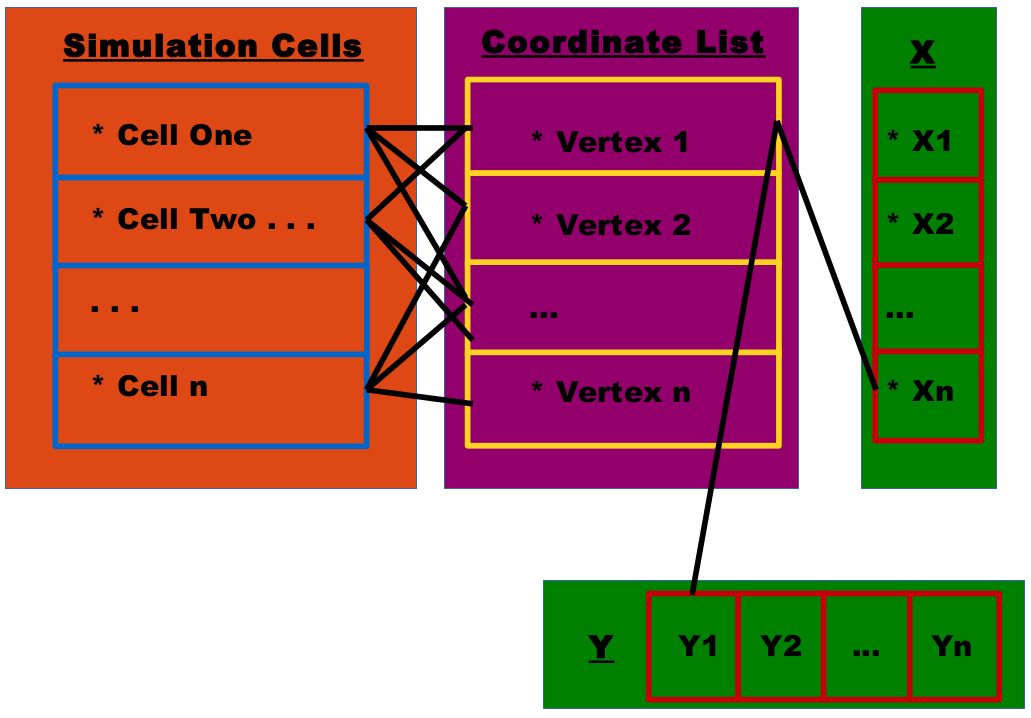
\includegraphics[width=0.5\textwidth]{../diagrams/ds.png}
\caption{The Relational Database}
\end{figure}

My data structure is inspired by the relational database model. I have six tables, including the simulationCells, coordinateList, X, Y, tempX and tempY tables. The cell and coordinate tables are implemented as 1d vectors of cell and coordinate indices, whereas the position tables are implemented as 1d arrays for ease of passing these structures to CUDA C functions (will talk more about CUDA C later). The cells can extract coordinate information from the coordinateList table via the \emph{index} key, and the coordinateList can access the position information from the X and Y arrays via their own \emph{index}. The temporary X and Y arrays store temporary position information about the vertices before the mesh positions are updated. This choice saves memory because the cells, coordinates, and coordinate locations are stored independently of each other, and there is no data redundancy. 

\section{Moving the Vertices}
\emph{GrowFlesh} loops over the vertices, computes the force applied to each vertex and then computes a displacement due to the force using the Euler Method. In their original paper, H. Honda and T. Nagai described the use of a Modified Runge Kutta Method to move the vertices, but this method would result in extra unnecessary computations at each time step. The \emph{Error Tolerance} section of this chapter describes how the Euler Method is numerically stable enough for this application. The same decision to use then Euler Method was made by the research group at Oxford that developed CHASTE, the \emph{other} leading software for implementing the Nagai-Honda Model. 

A displacement is calculated and stored in the temporary X and Y arrays. No vertex is permitted to move more than one half of the minimum delta separating vertices (the $\delta$ under which a T1 swap will occur) during an integration. By imposing this restiction we are ensuring that we will not miss the event of two vertices coming critcally close and a T1 swap occurring. Also, this prevents vertices from passing each other and invalidating the mesh. To ensure that no vertex moves too much, we store verify each displacement as we put it in the temporary X and Y arrays. If a displacement is too large, then the entire array of temporary displacements is erased, the time step is halved, and we begin the integration again. We could label the integrator as `fault tolerant'.

\begin{wrapfigure}{L}{0.4\textwidth}
\begin{center}
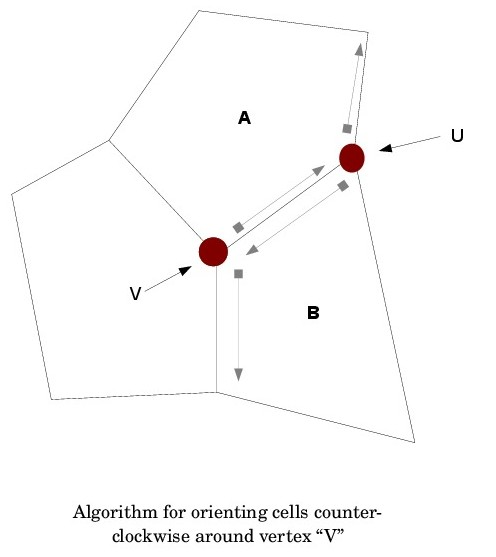
\includegraphics[width=0.38\textwidth]{../diagrams/counterclockwise.jpg}
\end{center}
\caption{Getting Cells in Order}
\label{fig:ctrclockwise}
\end{wrapfigure}

Another important aspect of the numerical integration is that cell and vertex information must be processed in counterclockwise order. In Figure~\ref{fig:ctrclockwise} I illustrate how a vertex can find the cells surrounding it in this order. When we are integrating a vertex $i$, the vertex first searches in the cell vector for a cell which contains it, and then the vertex finds the next vertex in that cell. Then, we have an edge. Some other cell contains that edge if it contains both of the vertices. That cell must be clockwise from the first. The cells are stored in the reverse order of which they are uncovered by this algorithm before the integration starts. This is a very expensive step ($O(n^3)$) in the computation, and ought to be optimized.


\section{Embarassing Parallelism and CUDA}
The numerical integrations and the vertex location updates exhibit what Cleve Moler describes as ``embarassing parallelism''. Computing the displacement of vertex \emph{a} does not depend upon the computation of the displacement of vertex \emph{b} during a given time step. Similarly, the vertex locations can all be updated in parallel since the update is simply a vector sum operation of the X and Y arrays with the temporary X and Y arrays, respectively. 

A popular hardware choice for parallel programming in last decade has been the NVIDIA GPU. CUDA is the NVIDIA extension of the C programming language which can run certain parts of C code on the GPU, while still running the serial and i/o operation on the CPU. I wrote some parts of the code in this language, and these parts were very simple to implement. The GPU is a collection of small processors, and the vertices are small, simple objects, so I mapped each vertex in the mesh to one of the hundreds of small processors to get some computational speedup.

Specifically, CUDA was employed to update vertex locations, since the sum of 1d arrays is well suited to a GPU. I also parallelized the rotation of the mesh and the reduction step which found the maximum error between the mesh and the rotated mesh. An interesting possibility is that of parallelizing the force computations. I was unable to do this with the code as it is because the cell data uses C++ vectors, while cuda only likes to take large C arrays as input. There is an interesting library called \emph{thrust} which can strips the vectors down to arrays and does all of the memory allocations for you, but the issue then becomes one of compiling the cells into one big vector with clever structure. This is left as a future project. 

CUDA was used to multiply each vertex in the mesh by the rotation matrix:
\[ \left( \begin{array}{cc}
\cos\theta & -\sin\theta \\
\sin\theta & \cos\theta 
\end{array} \right)\] 

\section{Computing Topological changes.}
\subsection{The T1 Swap}
The PerformT1s() function loops over all of the cells in the mesh, and checks the edge lengths in that cell. If an edge is critically small, then the other three cells involved in the junction are found. One of the two clashing vertices is deleted from the main cell, and the other clashing vertex is deleted from the neighboring cell. The midpoint of the critical edge is calculated, and then a perpendicular line is drawn through it. The vertices are then moved a distance $\delta/2$ into the interior of the cells ($\delta$ is the minimum vertex separation, and the vertices now have this minimal spacing). Then, these two vertices are inserted into the cells which previously hadn't been neighbors, making then adjacent after the swap. Figure ~\ref{fig:t1} offers a visual aid to understanding the swap. 

There are 8 cases to consider when inserting moving the vertices the distance $\delta/2$. I and Ip1 are the critically close vertices, where Ip1 comes before I in clockwise order in a cell. $mp$ is the midpoint of $\bar{(I, Ip1)}$. $dx$ and $dy$ are the displacements which will give a minimal separation after the swap. 
\begin{enumerate}
\item %1
\textbf{Given:}\\
I.x $<$ Ip1.x AND I.y == Ip1.y
\textbf{Then:}\\
I $\mapsto$ mp + (0, -dy) AND Ip1 $\mapsto$ mp + (0, dy)
\item %2
\textbf{Given:}\\
I.x $>$ Ip1.x AND I.y == Ip1.y
\textbf{Then:}\\
I $\mapsto$ mp + (0, dy) AND Ip1 $\mapsto$ mp + (0, -dy)
%%%%%%%%%%%%%%%%%%%%%%%%%%%%%%%%%%%%%%%%%%%%%%%%%%%%%%%%%%%
\item %3
\textbf{Given:}\\
I.x $<$ Ip1.x AND I.y $<$ Ip1.y
\textbf{Then:}\\
I $\mapsto$ mp + (dx, -dy) AND Ip1 $\mapsto$ mp + (-dx, dy)
\item %4
\textbf{Given:}\\
I.x $>$ Ip1.x AND I.y $>$ Ip1.y
\textbf{Then:}\\
I $\mapsto$ mp + (-dx, dy) AND Ip1 $\mapsto$ mp + (dx, -dy)
%%%%%%%%%%%%%%%%%%%%%%%%%%%%%%%%%%%%%%%%%%%%%%%%%%%%%%%%%%%
\item %5
\textbf{Given:}\\
I.x $<$ Ip1.x AND I.y $>$ Ip1.y
\textbf{Then:}\\
I $\mapsto$ mp + (-dx, -dy) AND Ip1 $\mapsto$ mp + (dx, dy)
\item %6
\textbf{Given:}\\
I.x $>$ Ip1.x AND I.y $<$ Ip1.y
\textbf{Then:}\\
I $\mapsto$ mp + (dx, dy) AND Ip1 $\mapsto$ mp + (-dx, -dy)
%%%%%%%%%%%%%%%%%%%%%%%%%%%%%%%%%%%%%%%%%%%%%%%%%%%%%%%%%%%
\item %7
\textbf{Given:}\\
I.x == Ip1.x AND I.y $>$ Ip1.y
\textbf{Then:}\\
I $\mapsto$ mp + (dx, -dy) AND Ip1 $\mapsto$ mp + (-dx, dy)
\item %8
\textbf{Given:}\\
I.x == Ip1.x AND I.y $<$ Ip1.y
\textbf{Then:}\\
I $\mapsto$ mp + (dx, -dy) AND Ip1 $\mapsto$ mp + (-dx, dy)
\end{enumerate}

\subsection{The implementation of the T2 swap.}
The PerformT2s() function looks at every cell in the mesh and checks its area. If the area is critically small, then the cell is deleted from the mesh. The centroid of the triangle is calculated, and this become the collapsed triangle. Then, one of the three vertices has its position updated to the centroid coordinate and any cell which contained on of the other two coordinates is assigned the centroid coordinate index as a replacement.

\section{Error Tolerance of the Algorithm}
\emph{GrowFlesh} has been empirically shown to be numerically stable; the code outputs an error measurement at the end of a simulation to give the user a sense of the stability. There was no clear way to provide an analytical proof of stability but at least we will always have an error measure to strengthen our confidence in the code. \emph{GrowFlesh} runs two simultions at the same time, one on the mesh made by hex\_mesh(), and another on the same mesh which has been rotated 45 degrees. Then, at the end of a simulation, the rotated mesh is rotated back and corresponding vertices are compared by index using the Euclidean norm. In practice we see near machine epsilon error for every simulation.

\begin{figure}[hr]
\centering
\includegraphics[width=0.5\textwidth]{../Images/rotate.png}
\caption{A Rotated Mesh for Error Analysis.}
\end{figure}
%\chapter{Interesting Details for the Programmer}

\begin{thebibliography}{1}
\bibitem{Yoshi} K. Bambardekar et. al. Direct Laser Manipulation Reveals the Mechanics of Cell Contacts In Vivo \emph{PNAS} \textbf{112} 1416-1421.
\bibitem{MechanicalFeedback} Buchmann, A. Alber, M., Zartman, J. \emph{ Sizing it up: The mechanical feedback hypothesis of organ growth regulation.} Seminars in Cell and Developmental Biology, 2014.
\bibitem{Chaste Tutorial} \emph{Chaste Tutorial} \url{https://chaste.cs.ox.ac.uk/chaste/tutorials/release_2.1/UserTutorials.html}
\bibitem{Drasdo} Drasdo, D. \emph{Bucking Instabilities of One Layered Growing Tissues.} Physical Review Letters 84.
\bibitem{DurandStone} Durand, M., Stone, H. Relaxation Time of the Topological T1 process in a Two Dimensional Foam. arXiv.0
\bibitem{Epithelium}\emph{Epithelial Tissues} \url{http://www.botany.uwc.ac.za/sci_ed/grade10/mammal/epithelial.htm}
\bibitem{Farhadifar} Farhadifar, R., Roper, J., Algouy, B., Eaton, S., Jullcher, F. The Influence of Cell Mechanics, Cell-Cell Interactions, and Proliferation on Epithelial Packing. \emph{Current Biology} \textbf{17} 2095-2104. (2007) 
\bibitem{Vertex Models} Fletcher, A. , Osterfield, M., Baker, R., Shvartsman, S. \emph{Vertex Models of Epithelial Morphogenesis.} Biophysical Journal 106, June 2014.
\bibitem{ChasteMain} Fletcher, A., Osborne, J., Maini, P, Gavaghan, D. \emph{Implementing vertex dynamics models of cell populations in biology within a consitent computational framework.} Prog. Biophys. Mol. Biol. 113: 299 - 326.
\bibitem{Overview} Gibson, W., Gibson, M. \emph{Cell Topology, Geometry, and Morphogenesis  in Proliferating Epithelia.} Current Topics in Developmental Biology \textbf{89} 87-114. (2009)
\bibitem{Orientation} T. Gillies and C. Cabernard. Cell Division and Orientation in Animals. \emph{Current Biology} \textbf{21} 599-609
\bibitem{Relaxation of T1} P. Grassia, C. Oguey, R. Saepitomi. Relaxation of the topological T1 process in a two-dimensional foam. \emph{The European Physical Journal E} \textbf{35} (2012)
\bibitem{Dirichlet Domains} H. Honda. Description of Cellular Patterns by Dirichlet Domains: The Two-Dimensional Case. \emph{Journal of Theoretical Biology} \textbf{72} 523-543. (1978)
\bibitem{Cell Division} H. Honda, H. Yamanaka, M. Dan-Sohkawa. A Computer Simulation of Geometrical Configurations During Cell Division. \emph{Journal of Theoretical Biology} \textbf{106} 423-435. (1984)
\bibitem{Shape Formation} Honda, H. Essence of Shape Formation in Animals. \emph{Forma}, \textbf{27} S1-S8. (2012)
\bibitem{1989 Kawasaki} K. Kawasaki, T. Nagai, K. Nakashima. Vertex models for two-dimensional grain growth. \emph{Philisophical Magazine Part B} \textbf{60} 399 - 421. (1989)
\bibitem{rose} K. Liu, S. Ernst, V. Lecaudey, O. Ronneberger. Epithelial Rosette Detection in Microscopic Images.
\bibitem{Udacity} Luebke, D. and Owens, J. \emph{Intro to Parallel Programming} \url{https://www.udacity.com/course/cs344} 2013.
\bibitem{CellSize} Marshall et. al. What Determines Cell Size? \emph{BMC Biology} \textbf{10} (2012)
\bibitem{Wound Healing} T. Nagai and H. Honda. Wound Healing Mechanism in Epithelial Tissues Cell Adhesion to Basal Lamina. \emph{Proceedings of the 2006 WSEAS Int. Conf. on Cellular \& Molecular Biology, Biophysics \& Bioengineering}\textbf{2006} (pp111-116)
\bibitem{HondaNagai} Nagai, T. Honda, H. A dynamic model for the formation of epithelial tissues. \emph{Philisophical Magazine, Pt. B.}\textbf{81}(2001) 
\bibitem{Epithelial Topology} R. Nagpal, A. Patel, M. Gibson. Epithelial Topology. \emph{BioEssays} \textbf{30} 260-266. (2008)
\bibitem{Scaling Behavior} K. Nakashima, T. Nagai, K. Kawasaki. Scaling Behavior of Two-Dimensional  Domain Growth: Computer Simulation of Vertex Models. \emph{Journal of Statistical Physics} \textbf{57} 759-787. (1989)
\bibitem{TopStruct2DUnordered} Ohlenbusch, H.M., Aste, T. Dubertret, B., Rivier, N. The Topological Structure of 2D Disordered Cellular Structures. arXiv.
\bibitem{Okuda1} S.Okuda et. al. Reversible Network Reconnection Model for Simulating Large Deformation in Dynamic Tissue Morphogenesis. \emph{Biomech Model Mechanobiol} \textbf{12} 627-644 (2013)
\bibitem{epitheliumImage} \url{http://www.millerplace.k12.ny.us/webpages/lmiller/photos/636532/Epithelial\%20TissueTypes.bmp}
\bibitem{tutorvista} Potential Energy Graph \url{http://images.tutorvista.com/content/work-energy-power/potential-energy-variation.gif}
\bibitem{Order} K. Ragkousi and M. Gibson. Cell Division and the Maintenance of Epithelial Order. \emph{Journal of Cell Biology} \textbf{207} 181-188
\bibitem{Morphogen} Restrepo, S., Zartman, J. , and Basler, K. \emph{ Coordination of Patterning and Growth by the Morphogen DPP} Current Biology 24, 245- 255
\bibitem{Topological Models} R. Thom. Topological Models in Biology. \emph{Topology} \textbf{8} 313- 315 (1969)
\bibitem{Soap} Weaire, D. and Rivier, N. \emph{Soap, Cells, and Statistics}
\bibitem{Checkers} H. Yamanaka and H. Honda. A checkerboard pattern manifested by the oviduct epithelium of the Japanese Quail. \emph{Int. J. Dev. Biol.} \textbf{34} 377-383.
\end{thebibliography}



\appendix
\label{appendix}
\chapter{Getting, Running, and Modifying the Code} 
\section{GitHub}
When you are working on a large project such as this one, it is a good idea to have some sort of version control system which tracks the changes you have made to your code, and to return to an earlier working version in case something  gets terrribly broken. Many people who do not know about version control will do just this, except they will ´save as' every couple of days. Unfortunately, this method is very space inefficient, as each time you `save as', you save your entire project. Roughly speaking, git saves only the small changes you have made between versions. Git is a popular version control  tool, and github is a popular place to store you files online.

The following instructions show you how to create and clone git repositories. The repository for \emph{GrowFlesh} can be found at \url{https://github.com/JulianCienfuegos/NAGAIHONDAMODEL}.

\subsection*{Get Your Files on GitHub}
\begin{itemize}
\item Go to github.com and sign up for an account
\item Make a new repo on github
\item cd to the directory of your project on your machine.
\item git init
\item git add .
\item git commit -m ``some message"
\item git remote add origin YOUR URL HERE (This url is given to you from github when you make the repo.)
\item git pull origin master
\item git push origin master
\end{itemize}

\subsection*{Access And Modify These Files Somewhere Else}
\begin{itemize}
\item Simply type git clone \url{url of repository here} into a terminal
\item Work on project
\item git push origin master, when done working.
\end{itemize}


\end{document}
